%
%DIF LATEXDIFF DIFFERENCE FILE
%DIF DEL 0330_paper.tex   Thu Mar 31 14:12:27 2016
%DIF ADD ../paper.tex     Fri Apr  1 04:11:25 2016
% File: thesis.tex
% Created: 月 11 30 08:00 午後 2015 東京 (標準時)
% Last Change: 月 11 30 08:00 午後 2015 東京 (標準時)
%
%%% jdummy.def
%
\DeclareRelationFont{JY1}{mc}{it}{}{OT1}{cmr}{it}{}
\DeclareRelationFont{JT1}{mc}{it}{}{OT1}{cmr}{it}{}
\DeclareFontShape{JY1}{mc}{m}{it}{<5> <6> <7> <8> <9> <10> sgen*min
    <10.95><12><14.4><17.28><20.74><24.88> min10
    <-> min10}{}
\DeclareFontShape{JT1}{mc}{m}{it}{<5> <6> <7> <8> <9> <10> sgen*tmin
    <10.95><12><14.4><17.28><20.74><24.88> tmin10
    <-> tmin10}{}
\DeclareRelationFont{JY1}{mc}{sl}{}{OT1}{cmr}{sl}{}
\DeclareRelationFont{JT1}{mc}{sl}{}{OT1}{cmr}{sl}{}
\DeclareFontShape{JY1}{mc}{m}{sl}{<5> <6> <7> <8> <9> <10> sgen*min
    <10.95><12><14.4><17.28><20.74><24.88> min10
    <-> min10}{}
\DeclareFontShape{JT1}{mc}{m}{sl}{<5> <6> <7> <8> <9> <10> sgen*tmin
    <10.95><12><14.4><17.28><20.74><24.88> tmin10
    <-> tmin10}{}
\DeclareRelationFont{JY1}{mc}{sc}{}{OT1}{cmr}{sc}{}
\DeclareRelationFont{JT1}{mc}{sc}{}{OT1}{cmr}{sc}{}
\DeclareFontShape{JY1}{mc}{m}{sc}{<5> <6> <7> <8> <9> <10> sgen*min
    <10.95><12><14.4><17.28><20.74><24.88> min10
    <-> min10}{}
\DeclareFontShape{JT1}{mc}{m}{sc}{<5> <6> <7> <8> <9> <10> sgen*tmin
    <10.95><12><14.4><17.28><20.74><24.88> tmin10
    <-> tmin10}{}
\DeclareRelationFont{JY1}{gt}{it}{}{OT1}{cmbx}{it}{}
\DeclareRelationFont{JT1}{gt}{it}{}{OT1}{cmbx}{it}{}
\DeclareFontShape{JY1}{mc}{bx}{it}{<5> <6> <7> <8> <9> <10> sgen*goth
    <10.95><12><14.4><17.28><20.74><24.88> goth10
    <-> goth10}{}
\DeclareFontShape{JT1}{mc}{bx}{it}{<5> <6> <7> <8> <9> <10> sgen*tgoth
    <10.95><12><14.4><17.28><20.74><24.88> tgoth10
    <-> tgoth10}{}
\DeclareRelationFont{JY1}{gt}{sl}{}{OT1}{cmbx}{sl}{}
\DeclareRelationFont{JT1}{gt}{sl}{}{OT1}{cmbx}{sl}{}
\DeclareFontShape{JY1}{mc}{bx}{sl}{<5> <6> <7> <8> <9> <10> sgen*goth
    <10.95><12><14.4><17.28><20.74><24.88> goth10
    <-> goth10}{}
\DeclareFontShape{JT1}{mc}{bx}{sl}{<5> <6> <7> <8> <9> <10> sgen*tgoth
    <10.95><12><14.4><17.28><20.74><24.88> tgoth10
    <-> tgoth10}{}
\DeclareRelationFont{JY1}{gt}{sc}{}{OT1}{cmbx}{sc}{}
\DeclareRelationFont{JT1}{gt}{sc}{}{OT1}{cmbx}{sc}{}
\DeclareFontShape{JY1}{mc}{bx}{sc}{<5> <6> <7> <8> <9> <10> sgen*goth
    <10.95><12><14.4><17.28><20.74><24.88> goth10
    <-> goth10}{}
\DeclareFontShape{JT1}{mc}{bx}{sc}{<5> <6> <7> <8> <9> <10> sgen*tgoth
    <10.95><12><14.4><17.28><20.74><24.88> tgoth10
    <-> tgoth10}{}
\DeclareRelationFont{JY1}{gt}{it}{}{OT1}{cmr}{it}{}
\DeclareRelationFont{JT1}{gt}{it}{}{OT1}{cmr}{it}{}
\DeclareFontShape{JY1}{gt}{m}{it}{<5> <6> <7> <8> <9> <10> sgen*goth
    <10.95><12><14.4><17.28><20.74><24.88> goth10
    <-> goth10}{}
\DeclareFontShape{JT1}{gt}{m}{it}{<5> <6> <7> <8> <9> <10> sgen*tgoth
    <10.95><12><14.4><17.28><20.74><24.88> tgoth10
    <-> tgoth10}{}
\endinput
%%%% end of jdummy.def

\documentclass{sig-alternate-05-2015}
%\usepackage[dvipdfmx]{graphicx}
\usepackage{amssymb}
\usepackage{enumerate,cite,url}
\usepackage{listings,jlisting}
\lstset{%
    language={c},%
    basicstyle={\small},%
    identifierstyle={\small},%
    commentstyle={\small\itshape},%
    keywordstyle={\small},%\bfseries},%
    ndkeywordstyle={\small},%
    stringstyle={\small\it},
    frame={tb},
    breaklines=true,
    columns=[l]{fullflexible},%
    numbers=left,%
    xrightmargin=0zw,%
    xleftmargin=3zw,%
    numberstyle={\scriptsize},%
    stepnumber=1,
    numbersep=1zw,%
    %lineskip=-0.5ex%
}

% Copyright
\setcopyright{acmcopyright}
% DOI
\doi{10.475/123_4}
% ISBN
\isbn{123-4567-24-567/08/06}
%Conference
\conferenceinfo{EMSOFT '16}{October 2--7, 2016, Pittsburgh, USA}
\acmPrice{\$15.00}

\title{\DIFdelbegin \DIFdel{mruby Bytecode Loader Using Bluetooth }\DIFdelend \DIFaddbegin \DIFadd{Bluetooth Loader for mruby Bytecode }\\ \DIFaddend in Multi-VM Environment}
\numberofauthors{3}
\author{
\alignauthor
Takuro Yamamoto\\
    \affaddr{Graduate School of Engineering Science, Osaka University}\\
    \affaddr{Osaka, JAPAN}\\
       % \affaddr{Wallamaloo, New Zealand}\\
       % \email{trovato@corporation.com}
\alignauthor
Hiroshi Oyama\\
    \affaddr{OKUMA Corporation}\\
    \affaddr{Aichi, JAPAN}\DIFaddbegin \\
       \DIFaddend % \affaddr{Dublin, Ohio 43017-6221}\\
       % \email{webmaster@marysville-ohio.com}
\alignauthor
Takuya Azumi\\
    \affaddr{Graduate School of Engineering Science, Osaka University}\\
    \affaddr{Osaka, JAPAN}\\
       % \affaddr{Hekla, Iceland}\\
       % \email{larst@affiliation.org}
}
%\author{Takuro Yamamoto}
%\date{\today}
%DIF PREAMBLE EXTENSION ADDED BY LATEXDIFF
%DIF UNDERLINE PREAMBLE %DIF PREAMBLE
\RequirePackage[normalem]{ulem} %DIF PREAMBLE
\RequirePackage{color}\definecolor{RED}{rgb}{1,0,0}\definecolor{BLUE}{rgb}{0,0,1} %DIF PREAMBLE
\providecommand{\DIFadd}[1]{{\protect\color{blue}\uwave{#1}}} %DIF PREAMBLE
\providecommand{\DIFdel}[1]{{\protect\color{red}\sout{#1}}}                      %DIF PREAMBLE
%DIF SAFE PREAMBLE %DIF PREAMBLE
\providecommand{\DIFaddbegin}{} %DIF PREAMBLE
\providecommand{\DIFaddend}{} %DIF PREAMBLE
\providecommand{\DIFdelbegin}{} %DIF PREAMBLE
\providecommand{\DIFdelend}{} %DIF PREAMBLE
%DIF FLOATSAFE PREAMBLE %DIF PREAMBLE
\providecommand{\DIFaddFL}[1]{\DIFadd{#1}} %DIF PREAMBLE
\providecommand{\DIFdelFL}[1]{\DIFdel{#1}} %DIF PREAMBLE
\providecommand{\DIFaddbeginFL}{} %DIF PREAMBLE
\providecommand{\DIFaddendFL}{} %DIF PREAMBLE
\providecommand{\DIFdelbeginFL}{} %DIF PREAMBLE
\providecommand{\DIFdelendFL}{} %DIF PREAMBLE
%DIF END PREAMBLE EXTENSION ADDED BY LATEXDIFF

\begin{document}
\maketitle
\begin{abstract}
In recent years, the productivity of embedded systems has \DIFdelbegin \DIFdel{become }\DIFdelend a problem due to their complexity and large-scale.
For the purpose of improving the productivity for embedded software development, the mruby on TECS framework has been proposed that is applied mruby (Lightweight Ruby) and supports component-based development.
In the current mruby on TECS, the mruby programs have to be compiled and linked every time the programs are modified because the mruby bytecodes are incorporated in the platform.
Moreover, while the framework supports multi-VM, developers need to be familiar with the functions of real-time operating systems to effectively execute multiple mruby programs in concurrent or/and parallel.
To improve the development efficiency, this paper proposes \DIFdelbegin \DIFdel{an mruby bytecode loader using Bluetooth }\DIFdelend \DIFaddbegin \DIFadd{a Bluetooth loader for mruby bytecode }\DIFaddend as an extension of mruby on TECS.
The loader executes two mruby bytecodes, mruby application bytecode and mruby library bytecode.
mruby application bytecode \DIFdelbegin \DIFdel{modified frequently is }\DIFdelend \DIFaddbegin \DIFadd{is modified frequently and }\DIFaddend sent from a host to a target device by developers.
mruby library bytecode modified infrequently is preserved beforehand with the platform in a storage/ROM device at the time of the first compilation.
In addition, multiple mruby programs cooperatively run in the proposed framework.
A RiteVM scheduler makes multitasking processing more easy-to-use than that of mruby on TECS.
Synchronization of starting multiple tasks is also implemented with Eventflag. 
Experimental results demonstrate the advantages of the proposed framework.
\end{abstract}

\DIFdelbegin %DIFDELCMD < \keywords{embedded software; script language; component based development;}
%DIFDELCMD < %%%
\DIFdelend \DIFaddbegin \keywords{embedded software; script language; component-based development;}
\DIFaddend \section{Introduction}
In these days, embedded systems have been required the high-quality and the high-performance.
Due to this trend, the complexity of embedded systems also increases and the scale is larger.
For example, IoT (Internet of Things) applications.
The low production cost and the short developing period of time are also needed.

An approach of efficient software development is to use component-based techniques.
CBD (Component-Based Development) is a design technique for constituting reusable components \cite{par:Crnkovic}.
Complex and large scale software systems can be developed efficiently using component-based techniques.
That is because software componentization provides high-reusability.
Verification of component-based systems has been researched \cite{par:Blaming} \cite{par:Verification}.
It also \DIFaddbegin \DIFadd{visualize the entire system due to component diagrams, and }\DIFaddend makes a system flexible in extensions and specification changes.
There are TECS \cite{par:TECS}, AUTOSAR \cite{url:AUTOSAR}, and SaveCCM \cite{par:SAVEapproach} as a typical component-based development for embedded systems 

In addition, another approach of efficient software development is to develop with script languages.
Most of current software are programmed in C language\DIFdelbegin \DIFdel{, and the development with C }\DIFdelend \DIFaddbegin \DIFadd{.
Development with C language makes the code size increase, and }\DIFaddend takes a high cost and more time to develop.
Script languages make software engineering more efficient and shorten a development period because script languages have high-productivity from their usability.
\DIFdelbegin \DIFdel{Java script, }\DIFdelend \DIFaddbegin \DIFadd{Ruby, JavaScript, }\DIFaddend Perl, Python, \DIFdelbegin \DIFdel{Lua and Ruby }\DIFdelend \DIFaddbegin \DIFadd{and Lua }\DIFaddend are well-known as representative script languages.

Although script languages are easy to use and read, their execution time are \DIFdelbegin \DIFdel{slower }\DIFdelend \DIFaddbegin \DIFadd{larger }\DIFaddend than C language's.
For embedded systems, the real-time properties such as estimation of \DIFdelbegin \DIFdel{worst-execution }\DIFdelend \DIFaddbegin \DIFadd{worst-case execution }\DIFaddend time are very important factors.
Therefore, it is difficult to apply the script languages to embedded systems.

mruby on TECS is a component-based framework for running script program \cite{par:mrubyonTECS}.
It is integrated two technologies.
One is mruby, which is a script language for embedded systems \cite{par:mruby}, \cite{url:mruby}.
The other is TECS (TOPPERS Embedded Component System), which is a component-based framework for embedded systems \cite{par:TECS} \cite{url:TOPPERS}.
mruby on TECS supports to effectively run mruby script language on embedded systems.
mruby on TECS also makes execution time 100 times faster than that of mruby.

%DIF < This paper proposes two additional features of mruby on TECS, mruby bytecode loader using Bluetooth and RiteVM scheduler.
%DIF > This paper proposes two additional features of mruby on TECS, Bluetooth loader for mruby bytecode and RiteVM scheduler.
mruby on TECS has several problems at present.
One of the problems is low software development efficiency.
mruby on TECS only supports a storage/ROM device to load mruby programs. 
%in the platform for LEGO MINDSTORMS EV3 \cite{par:EV3}.
For example, an SD card should be inserted and pulled out repeatedly, or a ROM should be rewritten if mruby programs are modified.
Developers should also restart an \DIFdelbegin \DIFdel{OS }\DIFdelend \DIFaddbegin \DIFadd{RTOS }\DIFaddend on a target device.
%Moreover, in the current system if developers attempt to run multiple tasks with the same priority, a task with first execution only runs and all other tasks do not run unless developers call the OS's function.
%In addition developers must prepare as many VMs as the number of tasks because one RiteVM supports only one task.
Moreover, although mruby on TECS has supported the multi-VM, developers need to call OS's function in order to execute multiple tasks.
These \DIFdelbegin \DIFdel{problem are a big burden on }\DIFdelend \DIFaddbegin \DIFadd{problems makes the burden heavy for }\DIFaddend developers.

This paper proposes an extended framework of mruby on TECS: \DIFdelbegin \DIFdel{an mruby bytecode loader using Bluetooth }\DIFdelend \DIFaddbegin \DIFadd{a Bluetooth loader for mruby bytecode }\DIFaddend and a RiteVM scheduler for fairly executing mruby programs.
To improve the development efficiency, the \DIFdelbegin \DIFdel{mruby bytecode loader using Bluetooth }\DIFdelend \DIFaddbegin \DIFadd{proposed framework }\DIFaddend enables developers to \DIFdelbegin \DIFdel{write }\DIFdelend \DIFaddbegin \DIFadd{implement }\DIFaddend the platform in a storage device only once at the beginning and to transfer mruby application \DIFdelbegin \DIFdel{codes }\DIFdelend \DIFaddbegin \DIFadd{programs }\DIFaddend from a host to a target device \DIFdelbegin \DIFdel{.
}\DIFdelend \DIFaddbegin \DIFadd{using the Bluetooth Loader.
A RiteVM is a virtual machine for mruby.
}\DIFaddend The RiteVM scheduler \DIFaddbegin \DIFadd{manages the execution of multiple RiteVMs, }\DIFaddend enables developers to \DIFdelbegin \DIFdel{run multitasking programs }\DIFdelend \DIFaddbegin \DIFadd{program multitasking }\DIFaddend more easily than mruby on TECS.
%Specifically, a periodic handler of switching tasks is implemented.
%This paper evaluates the proposed framework in term of data transfer rate, overhead of periodic handler and execution time.

{\mybf Contribution}: The proposed framework gives the contribution in the following points.
\begin{enumerate}
\item {\mybf To improve the software development efficiency:} Developers do not need to rewrite a storage/ROM device and also to restart an \DIFdelbegin \DIFdel{OS}\DIFdelend \DIFaddbegin \DIFadd{RTOS}\DIFaddend .
The loader supports the continuous loading, which saves the Bluetooth set-up time.
Therefore, the \DIFdelbegin \DIFdel{mruby bytecode loader using Bluetooth }\DIFdelend \DIFaddbegin \DIFadd{Bluetooth loader for mruby bytecode }\DIFaddend helps developers develop software.
\item {\mybf To effectively execute multiple mruby programs in concurrent or/and parallel:} Developers can \DIFdelbegin \DIFdel{execute }\DIFdelend \DIFaddbegin \DIFadd{implement }\DIFaddend multiple tasks without the knowledge of an RTOS because the RiteVM scheduler switches tasks cyclically.
\item {\mybf To synchronize the execution of multiple RiteVM tasks:} The proposed framework provides the synchronization of multiple RiteVM tasks (mruby applications).
\item {\mybf To focus on the benefits of component-based developments:} This paper shows the specific examples for the benefits of component-based development. 
\end{enumerate}

{\mybf Organization}: The paper is organized as follows.
Section \ref{sec:Background} introduces the basic technologies i.e. mruby, TECS and mruby on TECS.
Section \ref{sec:Design and Implementation} describes the design and implementation of the proposed framework in detail.
Section \ref{sec:Evaluation} evaluates the proposed framework, Section \ref{sec:Related work} discusses related work, and then Section \ref{sec:Conclusion} concludes this paper.

\section{Background}
\label{sec:Background}
Figure \ref{fig:proposed} shows the system model of the proposed framework.
The bytecodes are transferred from the host to the target device with Bluetooth.
The RiteVMs and mruby library are assumed to be prepared in advance.
Each bytecode is allocated to a RiteVM, respectively.
\DIFdelbegin \DIFdel{Developers can run bytecodes }\DIFdelend \DIFaddbegin \DIFadd{Bytecodes }\DIFaddend transferred with Bluetooth \DIFaddbegin \DIFadd{from the host can run }\DIFaddend in multitask.

\begin{figure}[t]
    \centering
    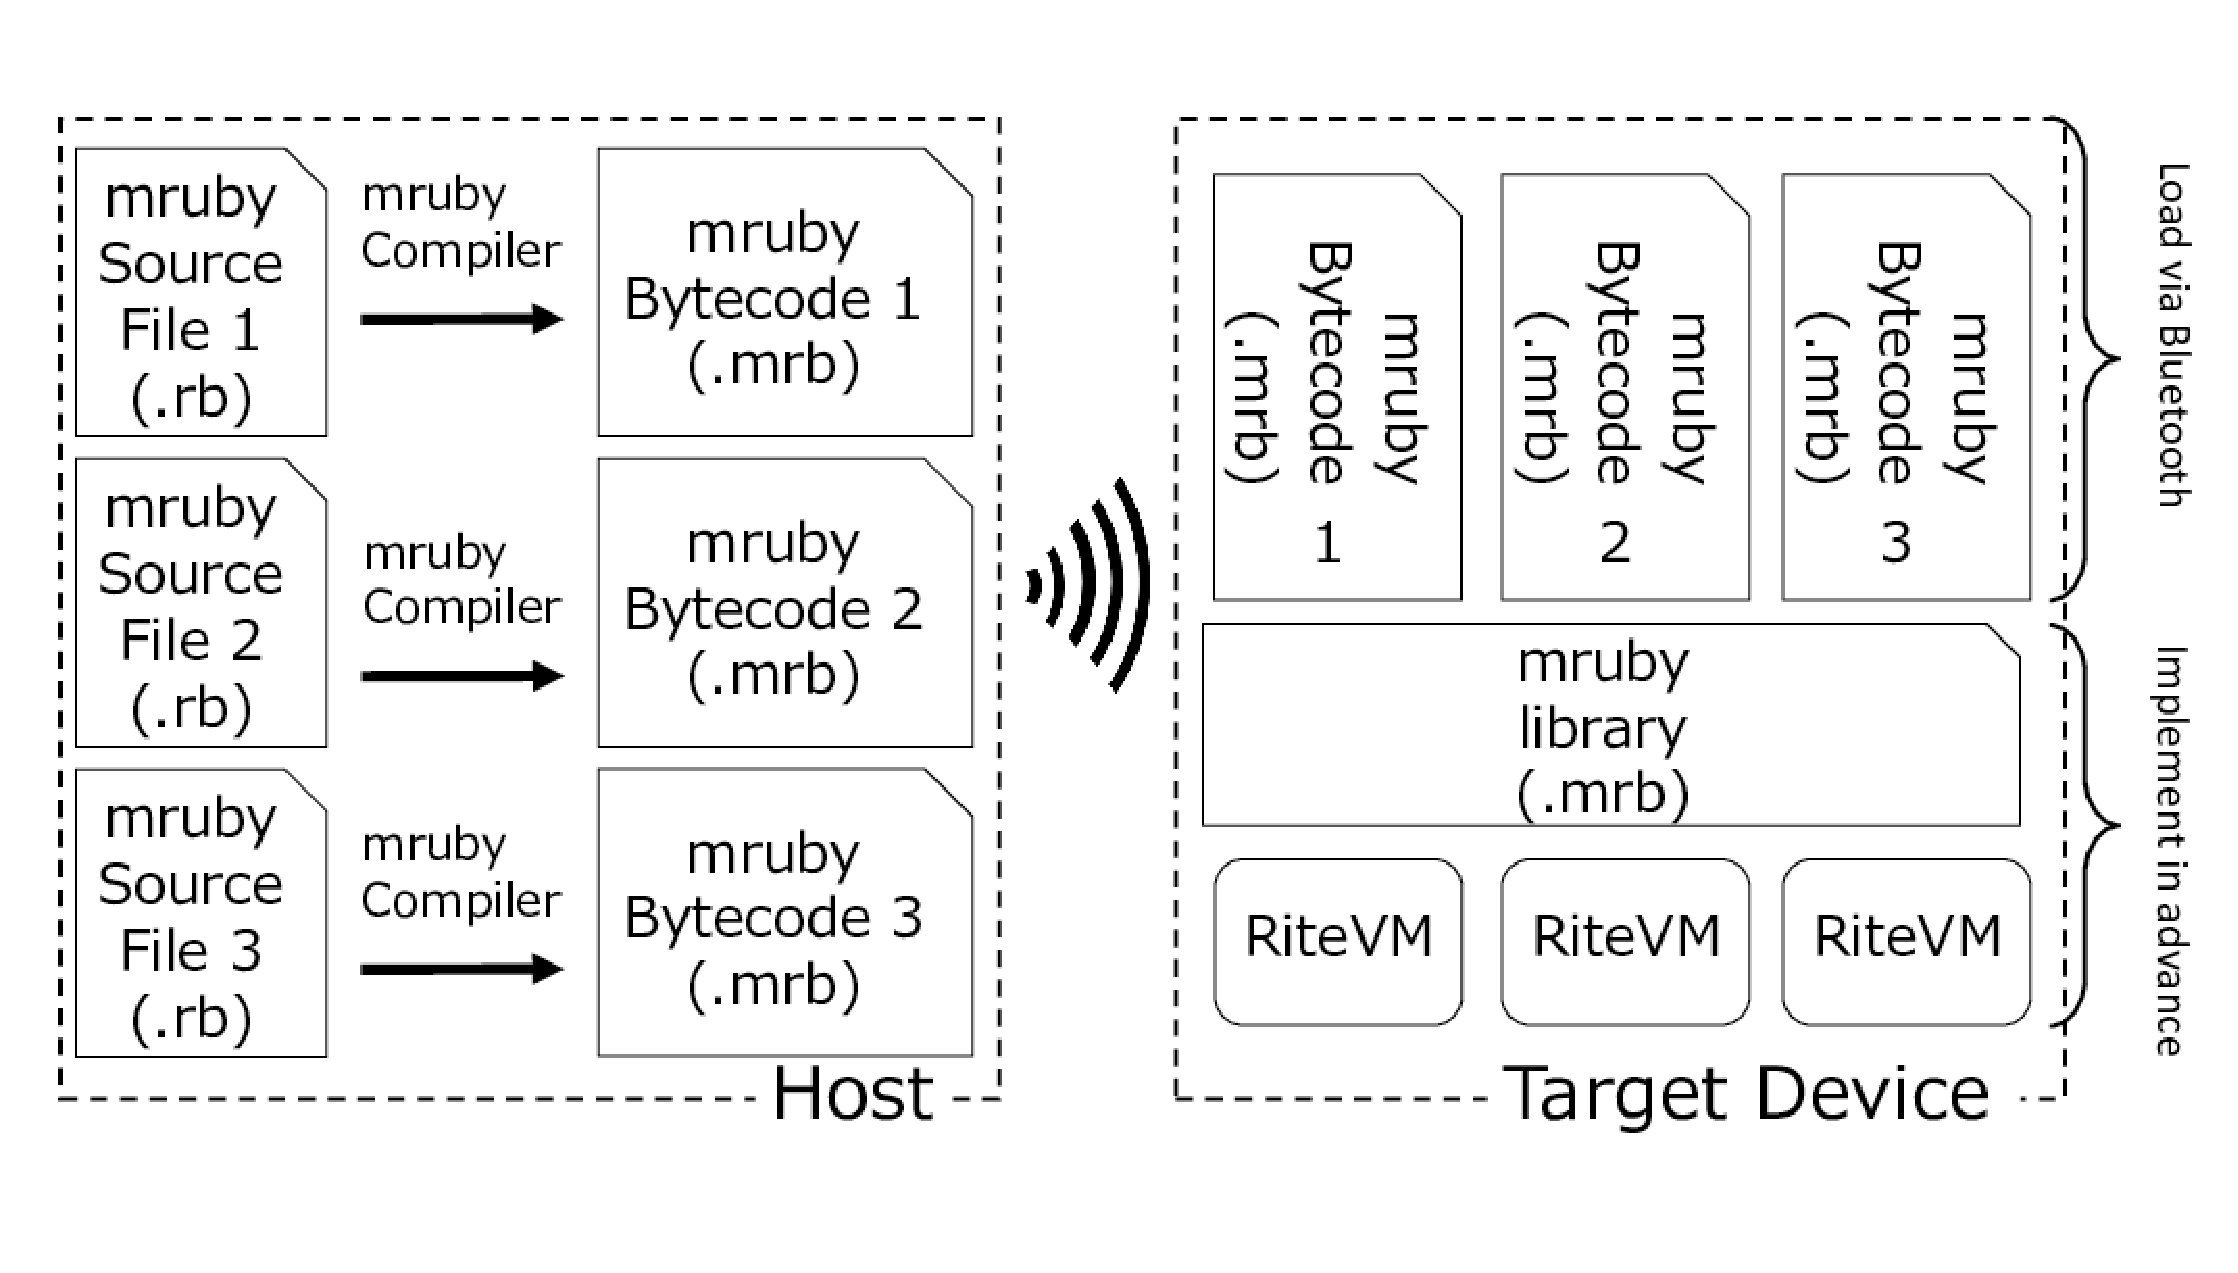
\includegraphics[width=8cm,clip]{figure/proposed.eps}
    \vspace{1mm}
    \caption{System Model of the proposed framework}
    \vspace{1mm}
    \label{fig:proposed}
\end{figure}

This section describes mruby on TECS on which the proposed framework is based.
mruby on TECS is a component-based framework for running script programs.
In mruby on TECS, two technologies are integrated: mruby and TECS.
To explain the system, mruby and TECS are also respectively described in this section.

\subsection{mruby}
\label{sec:mruby}
mruby is the light-weight implementation of Ruby programming language complying to part of the ISO standard.
Ruby is a object-oriented script language \cite{url:Ruby}.
As the main feature, Ruby is easy-to-use and easy-to-read due to its simple grammar.
Ruby can run a program with fewer code lines than C language.
Ruby improves the productivity of a software development owing to not only simple grammar but also object-oriented functions such as classes and methods, exceptions, and garbage collection.

mruby is suitable for embedded systems because of execution with less amount of resources and takes over the usability and readability of Ruby.
In addition, VM (Virtual Machine) mechanism is used in mruby, therefore mruby programs can run on any operating system as long as VM is implemented.
A RiteVM is a VM in mruby, that runs mruby programs.
The RiteVM mechanism is shown in Figure \ref{fig:mruby}.
The mruby compiler translates an mruby code into a bytecode, which is an intermediate code that can be interpreted by a RiteVM.
The bytecodes can run on a \DIFdelbegin \DIFdel{Rite VM}\DIFdelend \DIFaddbegin \DIFadd{RiteVM}\DIFaddend , and thus mruby programs can be executed on any target devices if only RiteVMs are implemented.
\begin{figure}[t]
    \centering
    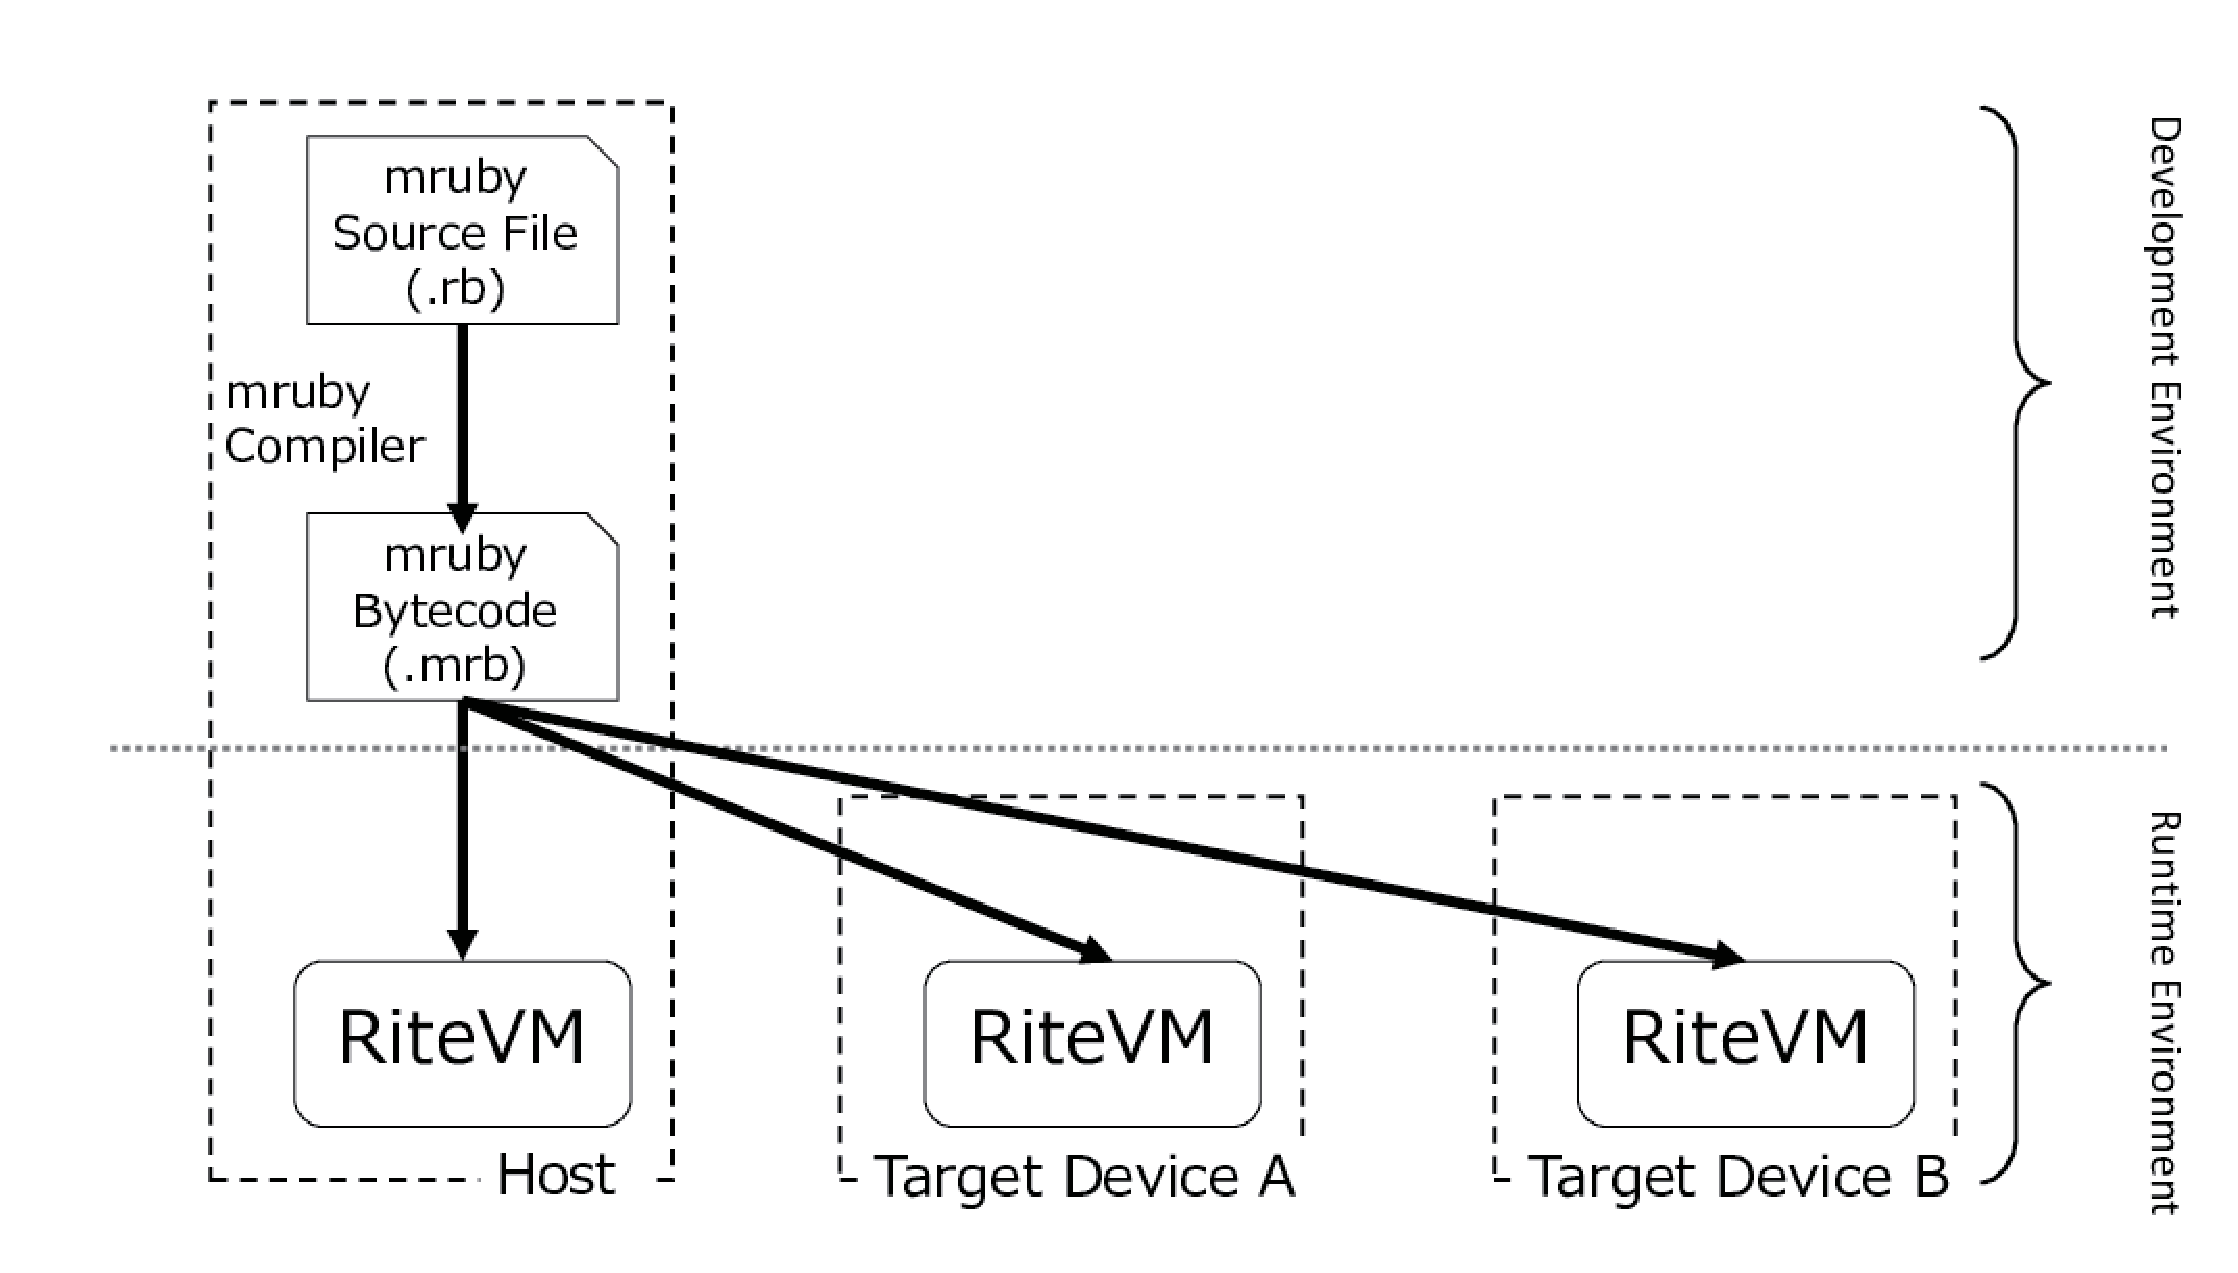
\includegraphics[width=8cm,clip]{figure/mruby.eps}
    \vspace{1mm}
    \caption{Mechanism of mruby/RiteVM}
    \vspace{1mm}
    \label{fig:mruby}
\end{figure}

\subsection{TECS}
\label{sec:TECS}
TECS \DIFdelbegin \DIFdel{(TOPPERS Embedded Component System) }\DIFdelend is a component system suitable for embedded systems.
TECS helps increase productivity and reduce development duplication because the reusability of software is improved.
TECS also helps \DIFdelbegin \DIFdel{decrease complexity of }\DIFdelend \DIFaddbegin \DIFadd{developers understand }\DIFaddend the system because the generated component diagram can visualize the structure of whole software.

The component deployment and composition in TECS are statically performed, which gives optimization.
As a result, the overhead of \DIFdelbegin \DIFdel{execution time and }\DIFdelend \DIFaddbegin \DIFadd{connection of components and the }\DIFaddend memory consumption can be reduced.
There are other features of TECS, implementation in C language, source level portability, fine-grained component, etc.

\subsubsection{Component Model}
Figure \ref{fig:component} shows a component diagram.
A {\myit cell} which is an instance of a component in TECS consists of {\myit entry} ports, {\myit call} ports, attributes and internal variables.
A {\myit entry} port is an interface to provide functions with other {\myit cell}s, and a {\myit call} port is an interface to use functions of other {\myit cell}s.
A {\myit cell} has one or more {\myit entry} ports and {\myit call} ports.
Functions of a {\myit cell} are implemented in the C language.

A type of a {\myit entry}/{\myit call} port is defined by a {\myit signature} which is a set of functions.
A {\myit signature} is the interface definition of a {\myit cell}.
The {\myit call} port of a {\myit cell} can be connected to the {\myit entry} port of another {\myit cell} with the same {\myit signature}.
A {\myit celltype} is the definition of a {\myit cell}.
{\myit Celltype} defines one or more {\myit call}/{\myit entry} ports, attributes and internal variables.

\begin{figure}[t]
    \centering
    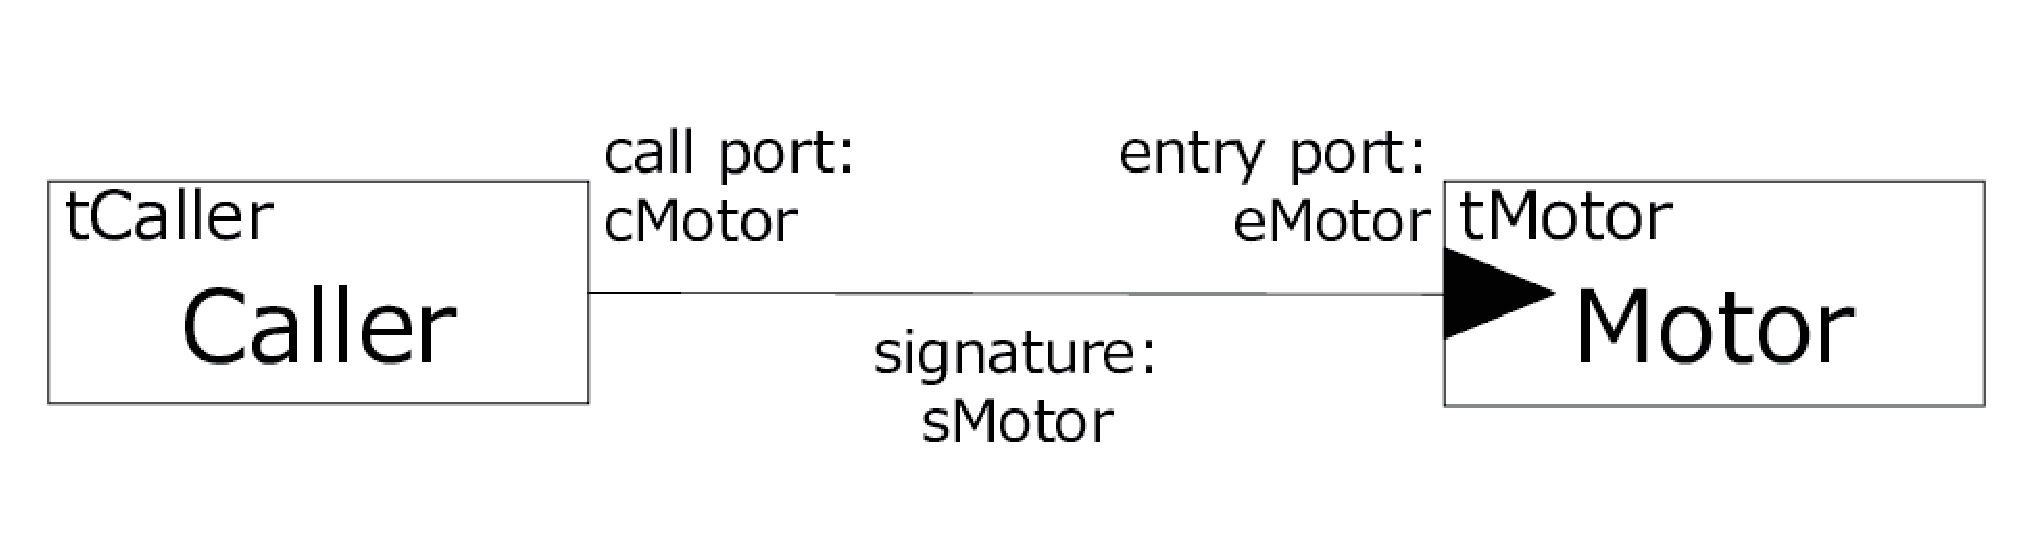
\includegraphics[width=8cm,clip]{figure/component_diagram.eps}
    \vspace{1mm}
    \caption{Component Diagram}
    \vspace{1mm}
    \label{fig:component}
\end{figure}

\subsubsection{Component Description}
The description of a component in TECS is divided into three parts, {\myit signature}, {\myit celltype}, and build description.
TECS code is written in \DIFdelbegin \DIFdel{.cdl }\DIFdelend \DIFaddbegin \DIFadd{CDL }\DIFaddend (component description language) file.
The component description is mentioned with an example shown in Figure \ref{fig:component} as follow.

\begin{description}
    \item[{\mybf Signature Description}]\mbox{}\\
        The {\myit signature} description defines an interface of a {\myit cell}.
        A {\myit signature} name is described following the keyword {\myit signature}.
        It also has the prefix ``s".
        In this way, a {\myit signature} is defined such as sMotor shown in Figure \ref{signature}.
        To make the definition of an interface clear, specifiers such as in and out are used in TECS.
        [in] and [out] represent input and output, respectively.
\begin{figure}[t]
\centering
\begin{lstlisting}
signature sMotor {
    int32_t getCounts( void );
    ER resetCounts( void );
    ER setPower( [in]int power );
    ER stop( [in] bool_t brake );
    ER rotate( [in] int degrees, [in] uint32_t speed_abs,
              [in] bool_t blocking );
    void initializePort( [in]int32_t type );
};
\end{lstlisting}
\vspace{1mm}
\caption{Signature Description}
\vspace{1mm}
\label{signature}
\end{figure}
    \item[{\mybf Celltype Description}]\mbox{}\\
        The {\myit celltype} description defines {\myit entry} ports, {\myit call} ports, attributes, and \DIFdelbegin \DIFdel{valuables }\DIFdelend \DIFaddbegin \DIFadd{variable }\DIFaddend of a {\myit celltype}.
        An example of a {\myit celltype} description is shown in Figure \ref{celltype}.
        A {\myit celltype} name following the keyword {\myit celltype} with the prefix ``t" and elements of a {\myit celltype} is described.
        To define {\myit entry} ports, a {\myit signature} such as sMotor, and an {\myit entry} port name such as eMotor follow the keyword {\myit entry}.
        In the same way, {\myit call} ports can be defined.
        Attributes and \DIFdelbegin \DIFdel{valuables }\DIFdelend \DIFaddbegin \DIFadd{variables }\DIFaddend follow the keyword {\myit attr} and {\myit var} respectively.
\begin{figure}[t]
\centering
\begin{lstlisting}
celltype tCaller {
    call sMotor cMotor;
};
celltype tMotor {
    entry sMotor eMotor;
    attr {
        int32_t port;
    };
    var {
        int32_t currentSpeed = 0;
    };
};
\end{lstlisting}
\vspace{1mm}
\caption{Celltype Description}
\vspace{1mm}
\label{celltype}
\end{figure}
    \item[{\mybf Build Description}]\mbox{}\\
        The build description is used to instantiate {\myit cell}s and connect {\myit cell}s.
        Figure \ref{build} shows an example of a build description.
        A {\myit celltype} name such as tMotor, and a {\myit cell} name such as Motor follow the keyword {\myit cell}.
        To compose {\myit cell}s, a {\myit call} port, a {\myit signature}, a {\myit entry} port in order are described.
        In this example, a {\myit entry} port eMotor in a {\myit cell} Motor is connected to a {\myit call} port cMotor in a {\myit cell} Caller.
        \DIFaddbegin \DIFadd{The }{\myit \DIFadd{C\_EXP}} \DIFadd{is the keyword to use macros defined in C files.
}

\DIFaddend \begin{figure}[t]
\centering
\begin{lstlisting}
cell tMotor Motor {
    \DIFaddbeginFL \DIFaddFL{port = C_EXP("PORT_A");
}\DIFaddendFL };
cell tCaller Caller {
    cMotor = Motor.eMotor;
};
\end{lstlisting}
\vspace{1mm}
\caption{Build Description}
\vspace{1mm}
\label{build}
\end{figure}

\end{description}

\subsection{mruby on TECS}
\label{sec:mruby on TECS}
mruby on TECS is a component-based framework for running script language.
This framework uses two technologies, mruby and TECS.

\subsubsection{System Model}
The system model of mruby on TECS is shown in Figure \ref{fig:mrubyontecs}.
Each mruby program, which is bytecode, runs on its own RiteVM as a componentized task of an RTOS.
TECS components support various embedded drivers such as motor and sensor drivers.

An mruby-TECS bridge plays a role to call a native program (e.g. C legacy code) from an mruby program.
The mruby-TECS bridge provides native libraries for mruby.
It also gives TECS components to receive the invocation from an mruby program.
The mruby-TECS bridge is described in more detail bellow.

As the target RTOS, TOPPERS/HRP2 \cite{url:HRP2}, \cite{par:hr-tecs} is used in this paper.
TOPPERS/HRP2 is an RTOS based on $\mu$ITRON \cite{par:microITRON} with memory protection.
However, mruby on TECS does not depend on the RTOS because TECS supports not only TOPPERS/HRP2 but also the other RTOSs such as OSEK \cite{par:OSEK} and TOPPERS/ASP \cite{par:ASP}, \cite{url:ASP}.

\begin{figure}[t]
    \centering
    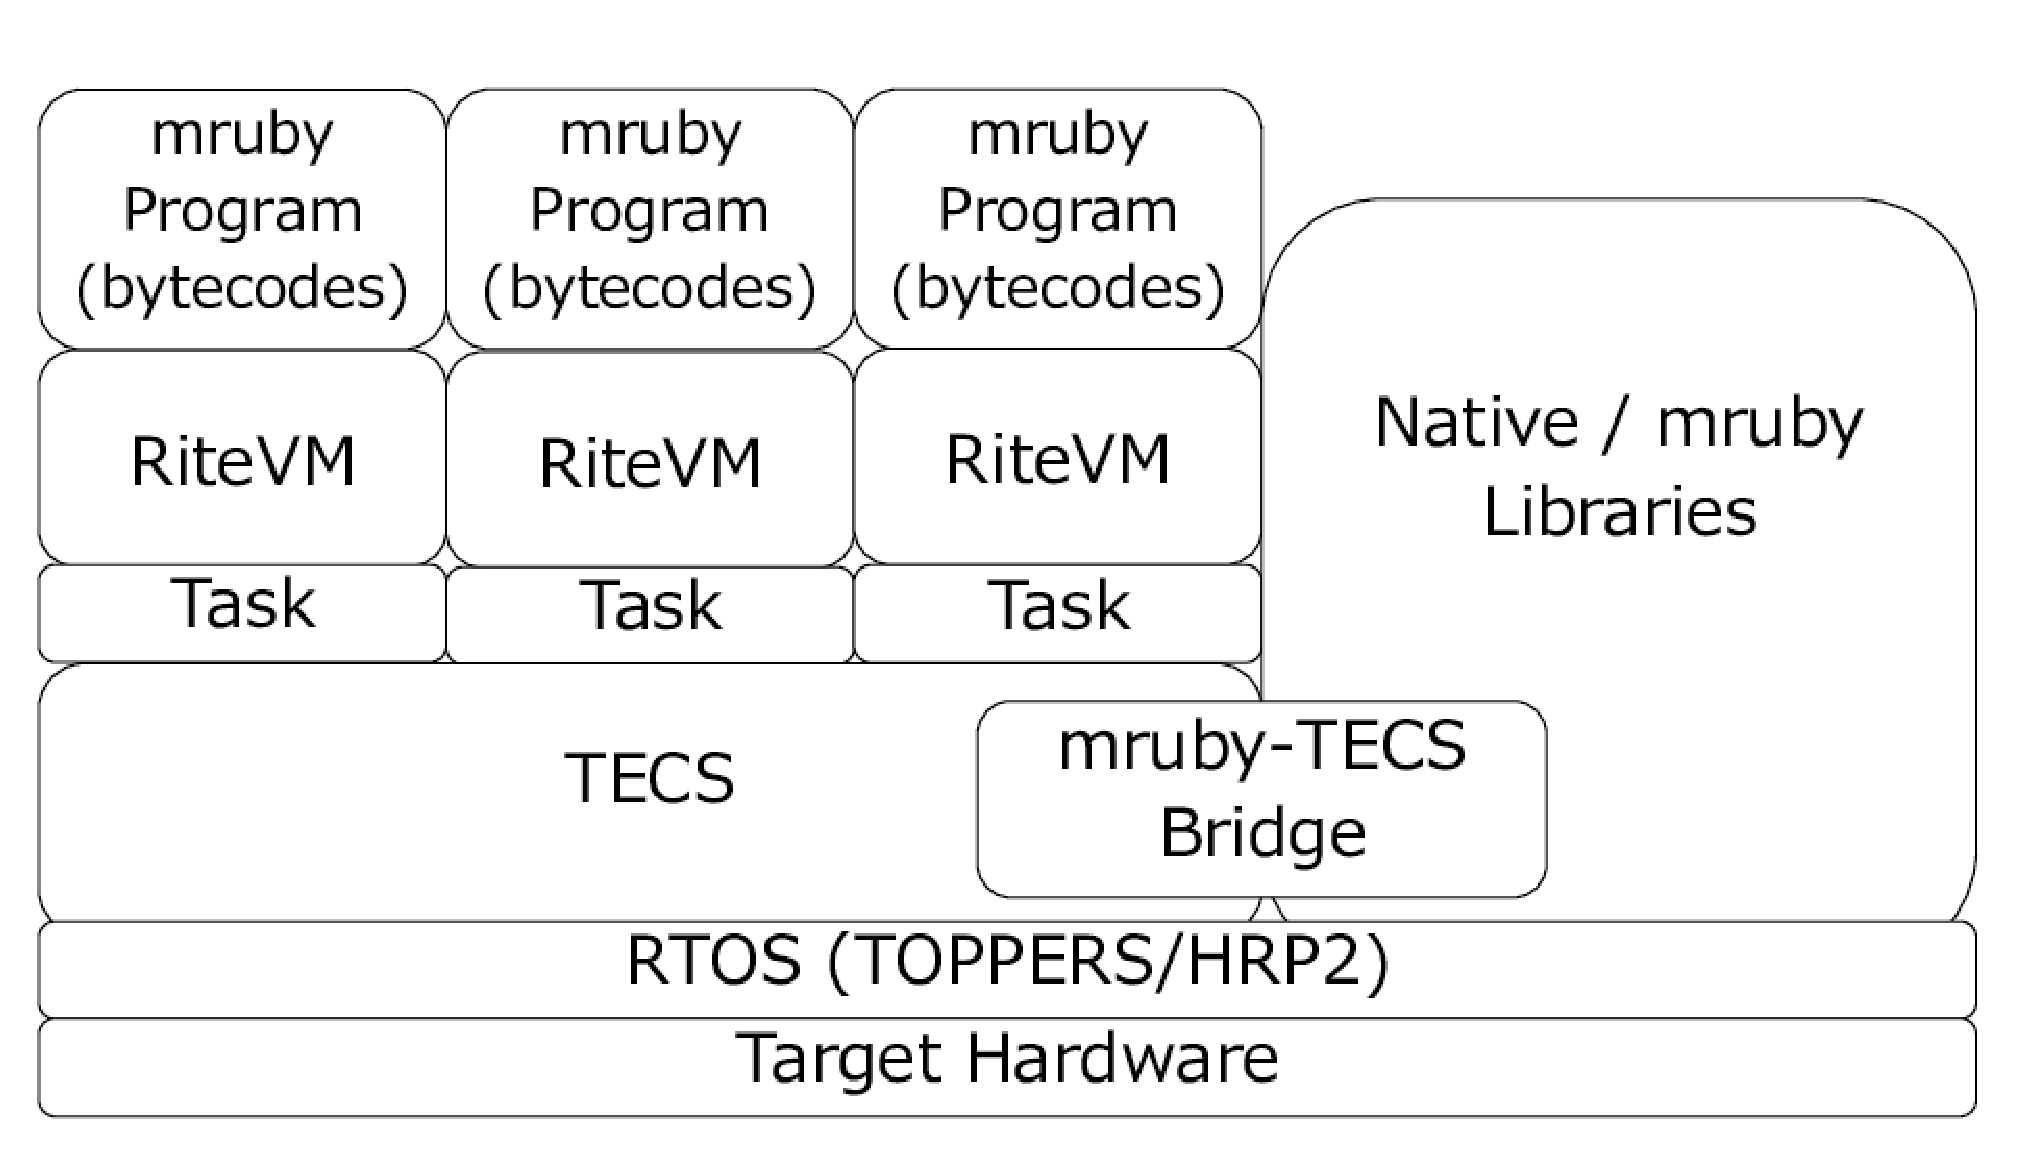
\includegraphics[width=8cm,clip]{figure/mrubyontecs.eps}
    \vspace{1mm}
\caption{System Model of existing mruby on TECS}
    \vspace{1mm}
\label{fig:mrubyontecs}
\end{figure}

\subsubsection{mruby-TECS Bridge}
There is a great difference between the execution time of mruby and C language.
According to  \cite{par:mrubyonTECS}, mruby programs are several hundreds times slower than C programs.
The execution of mruby bytecode on a RiteVM is not as efficient as that of C language.
Thus it is difficult to use mruby for all codes.

The use of Ruby on embedded devices provides the benefit of productivity and maintainability due to the ease to use and read.
On the other \DIFdelbegin \DIFdel{hands}\DIFdelend \DIFaddbegin \DIFadd{hand}\DIFaddend , it is necessary to implement parts of applications in C language in order to manipulate actuators and sensors, and also make a critical section of codes run quickly.

Figure \ref{fig:mruby_TECS_bridge} shows an example of use of an mruby-TECS bridge for controlling a motor.
The left side of BridgeMotor belongs to the mruby program.
The right side of BridgeMotor belongs to TECS component.
\begin{figure}[t]
    \centering
    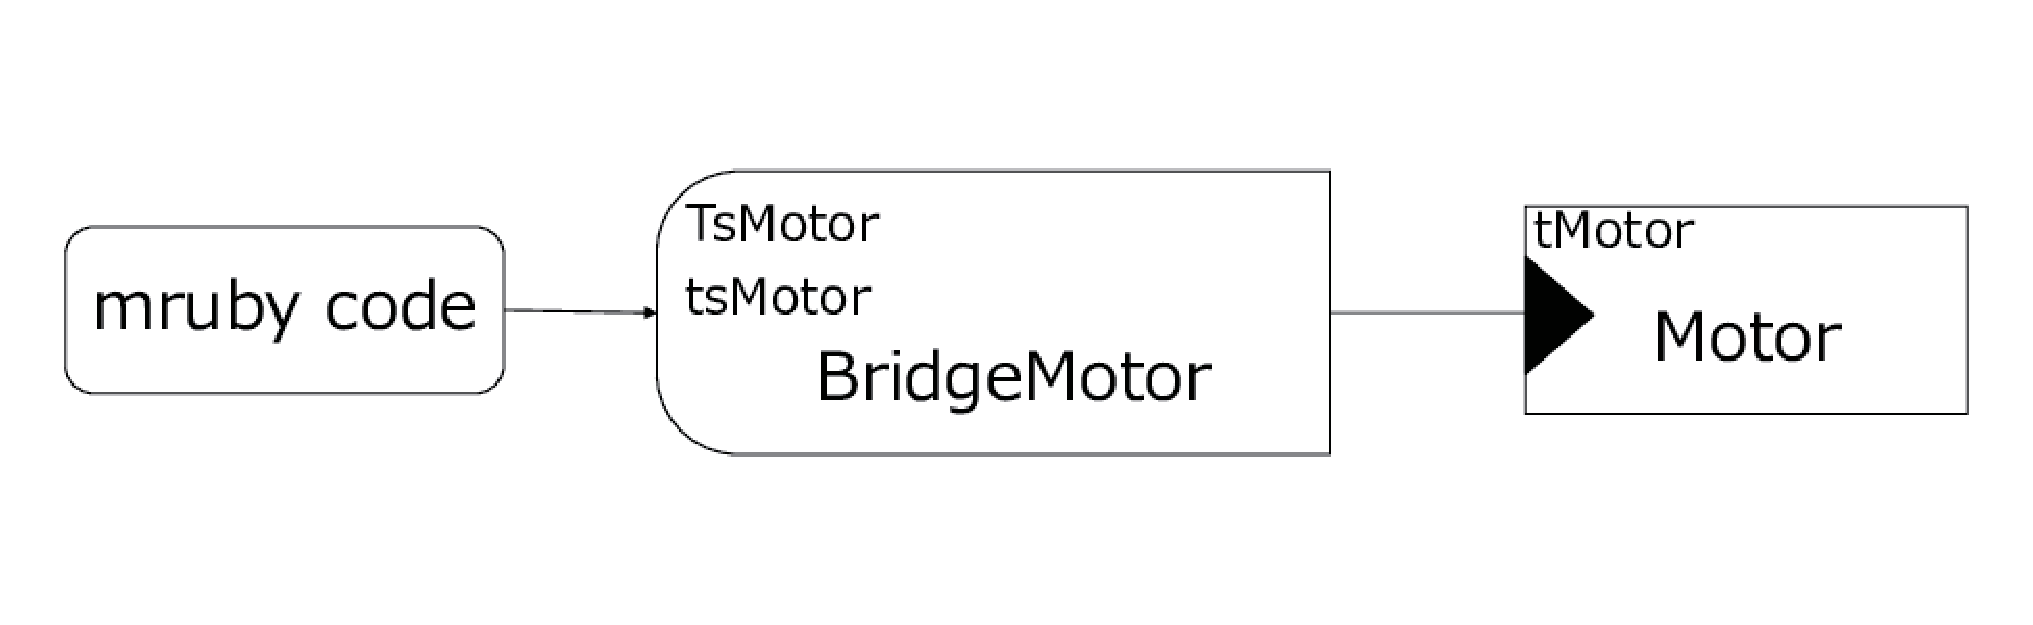
\includegraphics[width=8cm,clip]{figure/mruby_TECS_bridge.eps}
    \vspace{1mm}
\caption{mruby-TECS Bridge}
    \vspace{1mm}
\label{fig:mruby_TECS_bridge}
\end{figure}

The mruby-TECS bridge generates two things.
One is a {\myit celltype} to receive invocation from the mruby program.
The other is an mruby class that corresponds to the TECS component specified by the developers to invoke a C function from the mruby program.

A code of an mruby-TECS bridge is generated.
The generation code supports registration of classes and methods for mruby.
The methods in an mruby class are defined by generation codes for an mruby-TECS bridge, such as setPower and stop.
Thus, when a method is called in an mruby program, an mruby-TECS bridge calls the function defined in the TECS component such as a Motor {\myit cell}.

\section{Design and Implementation}
\label{sec:Design and Implementation}
Figure \ref{fig:system_model} shows the detailed system model of the proposed framework.
Each mruby application bytecode transferred from the host to the target \DIFdelbegin \DIFdel{deviceis }\DIFdelend \DIFaddbegin \DIFadd{devices }\DIFaddend received by the loader in the RiteVM.
The RiteVM reads the transferred bytecode and executes it with libraries.
The mruby applications run at the same time because of synchronization processing.
The RiteVM scheduler switches RiteVM tasks as multiple tasks can run in concurrent.
This section explains these proposed functionalities.

\begin{figure}[t]
    \centering
    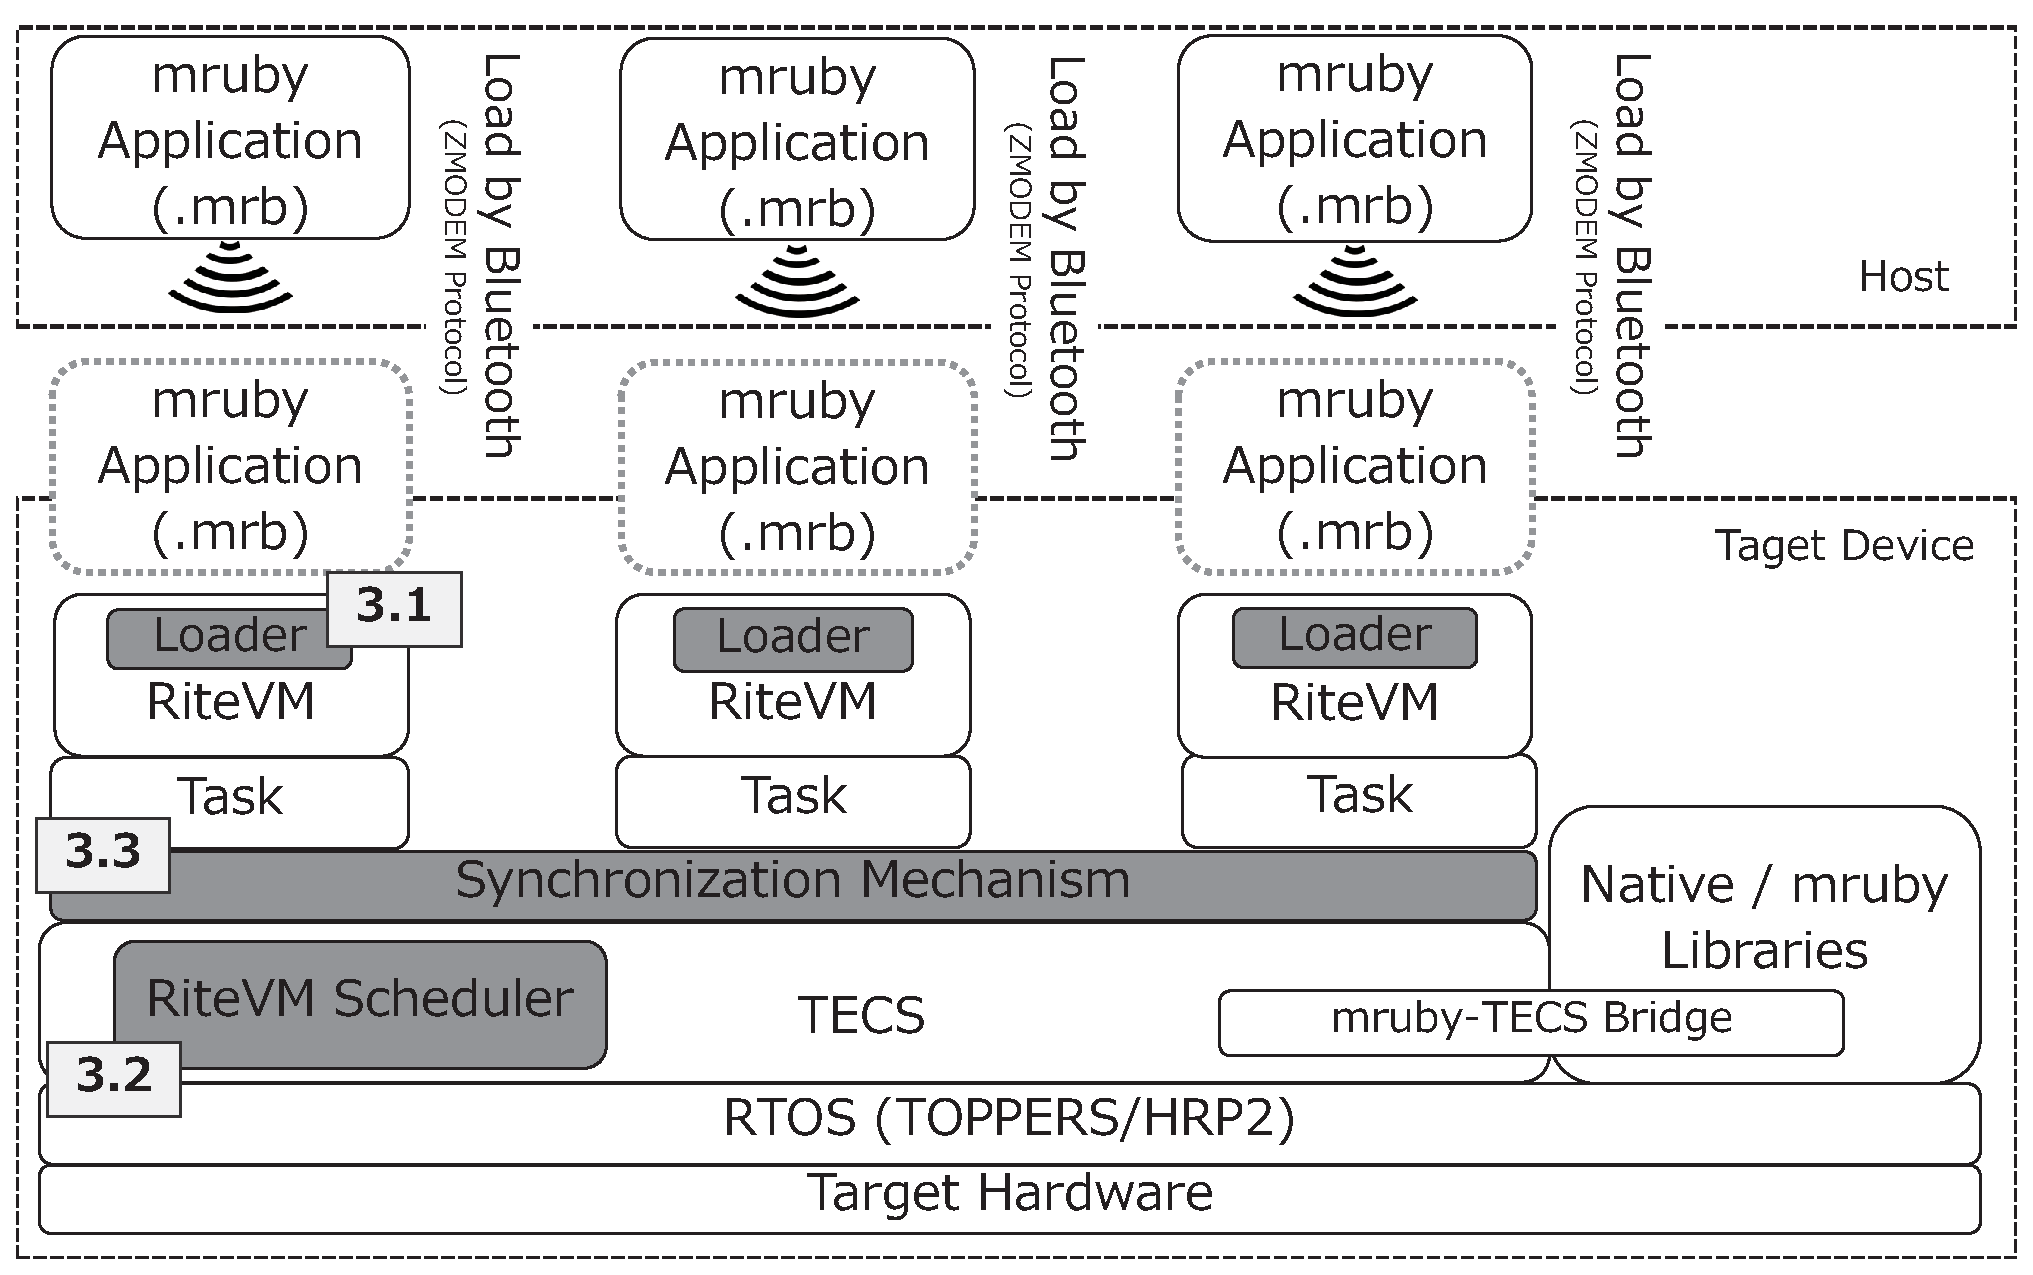
\includegraphics[width=8cm,clip]{figure/system_model.eps}
    \vspace{1mm}
\caption{Detailed System Model of the proposed framework}
    \vspace{1mm}
\label{fig:system_model}
\end{figure}

\subsection{\DIFaddbegin \DIFadd{Bluetooth Loader for }\DIFaddend mruby Bytecode\DIFdelbegin \DIFdel{Loader Using Bluetooth}\DIFdelend }
\DIFdelbegin %DIFDELCMD < \label{sec:mruby bytecode loader using Bluetooth}
%DIFDELCMD < %%%
\footnote{\DIFdel{mruby bytecode loader is intended to improve the development efficiency, therefore software developers should use it for development phase.
Complete software should be compiled and linked in the storage/ROM device beforehand.
}}
%DIFAUXCMD
\addtocounter{footnote}{-1}%DIFAUXCMD
\DIFdelend \DIFaddbegin \label{sec:Bluetooth loader for mruby bytecode}
\DIFaddend This section describes an additional functionality of mruby on TECS, \DIFdelbegin \DIFdel{mruby bytecode loader using Bluetooth.
}\DIFdelend \DIFaddbegin \DIFadd{Bluetooth loader for mruby bytecode.
}\footnote{
\DIFadd{Bluetooth loader is intended to improve the development efficiency, therefore software developers should use it for development phase.
Complete software should be compiled and linked in the storage/ROM device beforehand.
}}
\DIFaddend In the current system, the platform including mruby bytecodes are saved in a storage/ROM device.
Developers must rewrite the storage/ROM device every time the application programs are modified.
The \DIFdelbegin \DIFdel{OS }\DIFdelend \DIFaddbegin \DIFadd{RTOS }\DIFaddend on the target device should be also restarted.
It causes a low development efficiency to repeat that.
\DIFdelbegin \DIFdel{An mruby bytecode loader using Bluetooth }\DIFdelend \DIFaddbegin \DIFadd{A Bluetooth loader for mruby bytecode }\DIFaddend makes the developers' burden decrease.
%The work that an SD card is in and out needs to be done just once in the beginning.
Developers should just once carry out the work to connect the storage/ROM device and start the \DIFdelbegin \DIFdel{OS}\DIFdelend \DIFaddbegin \DIFadd{RTOS}\DIFaddend . 

mruby programs are consisted of mruby application and libraries.
mruby application is the main code which software developers should program.
mruby libraries are the codes defining the functions for application such as Ruby classes. 
The mruby bytecodes including mruby application and libraries can be sent and run.
However, it is also wasteful in terms of the size and time to send bytecodes because libraries are not frequently modified. 
The proposed framework provides the design that only mruby applications are sent and mruby libraries are preserved with the platform in the storage/ROM device beforehand.
Due to this design, RiteVMs can share the mruby libraries.
In addition, a RiteVM can use the own library that other RiteVMs should not use.

%DIF < The development flow in an mruby bytecode loader using Bluetooth is shown in Figure \ref{fig:bluetooth_loader}.
%DIF > The development flow in a Bluetooth loader for mruby bytecode is shown in Figure \ref{fig:bluetooth_loader}.
In the proposed framework, the platform including RiteVMs and mruby library is compiled and copied in the storage/ROM device at the first.
%These are assumed not to be modified.
%The binary data transferred with Bluetooth is the bytecode of the main source.
In the host, the mruby application programs (.rb) are edited and compiled into the bytecodes (.mrb) by an mruby compiler.
The generated bytecodes are transferred from the host to the target device with Bluetooth.

Moreover, developers can save the time of Bluetooth pairing since the loader can continuously load the bytecode.

% \begin{figure}[t]
%     \centering
%     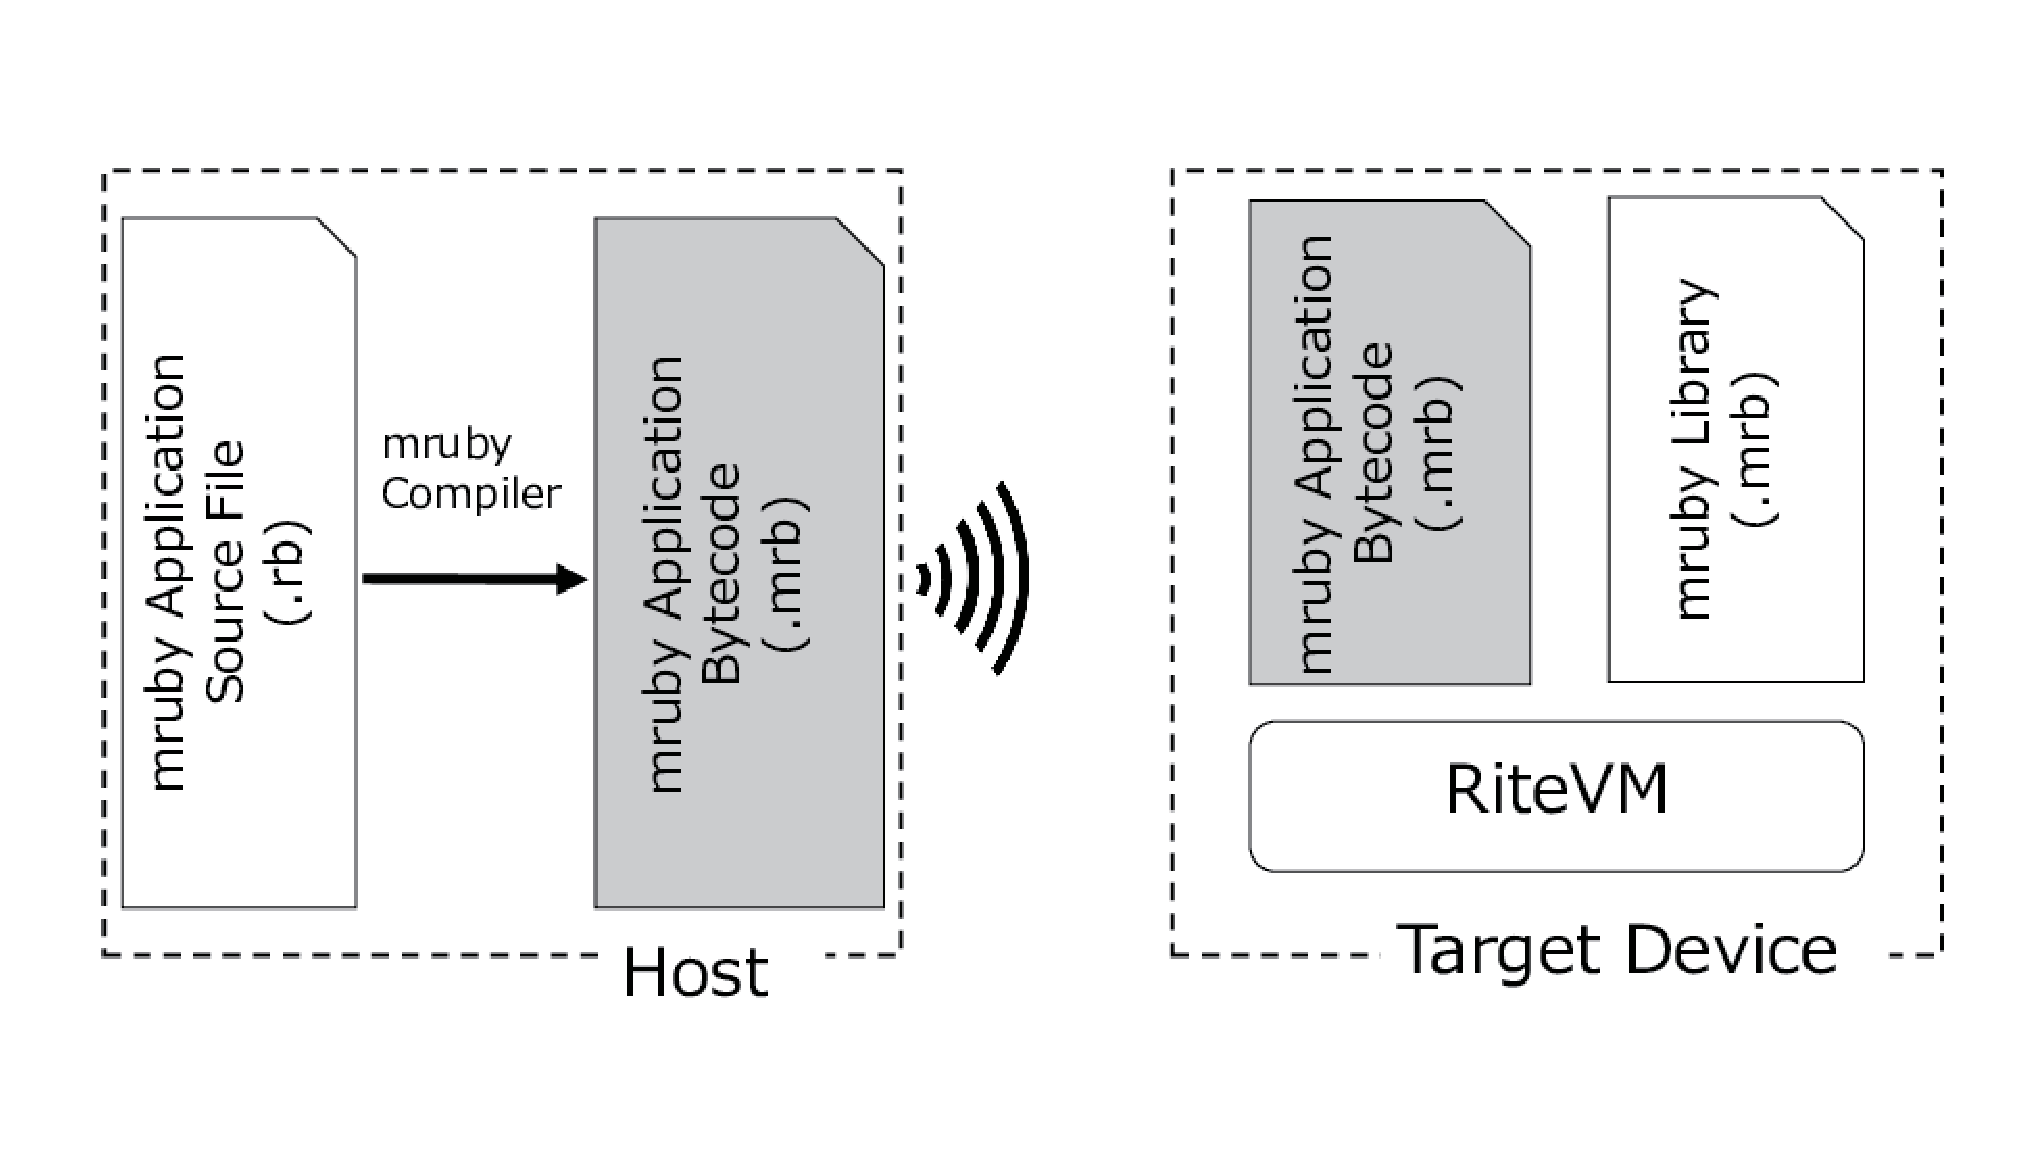
\includegraphics[width=8cm,clip]{figure/bluetooth_loader.eps}
%     \vspace{1mm}
%DIF <  \caption{Development Flow in mruby bytecode loader using Bluetooth}
%DIF >  \caption{Development Flow in Bluetooth loader for mruby bytecode}
%     \vspace{1mm}
% \label{fig:bluetooth_loader}
% \end{figure}

\subsubsection{Component of RiteVM with \DIFaddbegin \DIFadd{Bluetooth loader for }\DIFaddend mruby bytecode\DIFdelbegin \DIFdel{loader using Bluetooth}\DIFdelend }
\begin{figure}[t]
    \centering
    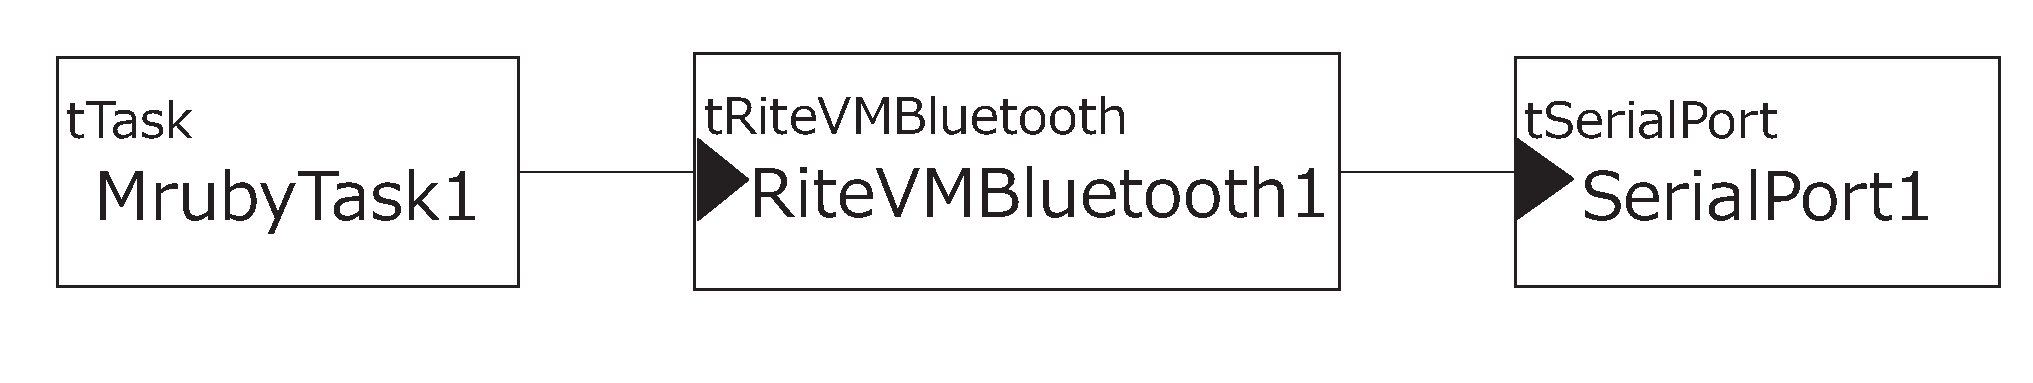
\includegraphics[width=8cm,clip]{figure/component_bluetooth.eps}
    \vspace{1mm}
\caption{Component Diagram of \DIFaddbeginFL \DIFaddFL{Bluetooth loader for }\DIFaddendFL mruby bytecode\DIFdelbeginFL \DIFdelFL{loader using Bluetooth}\DIFdelendFL }
    \vspace{1mm}
\label{fig:component_bluetooth}
\end{figure}
The proposed framework provides a RiteVM with \DIFdelbegin \DIFdel{mruby bytecode loader using Bluetooth }\DIFdelend \DIFaddbegin \DIFadd{Bluetooth loader for mruby bytecode }\DIFaddend as TECS component.
The component is an extension of the RiteVM component, which is described in \cite{par:mrubyonTECS}.
The component plays a role in receiving bytecodes via Bluetooth, and also manages a RiteVM configuration such as automatically \DIFdelbegin \DIFdel{generation }\DIFdelend \DIFaddbegin \DIFadd{generating }\DIFaddend the mruby library bytecode.
This generated bytecode is prepared beforehand in the storage/ROM device, and different from a bytecode transferred with Bluetooth.

Figure \ref{fig:component_bluetooth} shows a component diagram of MrubyTask1 and RiteVMBluetooth1 {\myit cell}s.
The MrubyTask1 {\myit cell} is a componentized task of the RTOS (TOPPERS/HRP2).
TOPPERS/HRP2 is described in \cite{url:HRP2}, \cite{par:hr-tecs}.
The RiteVMBluetooth1 is the component of RiteVM with \DIFdelbegin \DIFdel{mruby bytecode loader using Bluetooth}\DIFdelend \DIFaddbegin \DIFadd{Bluetooth loader for mruby bytecode}\DIFaddend .
A bytecode in the host is transferred and received at the top of the component.
In this framework, ZMODEM \cite{par:zmodem} is used as a binary transfer protocol.

\begin{figure}[t]
    \centering
    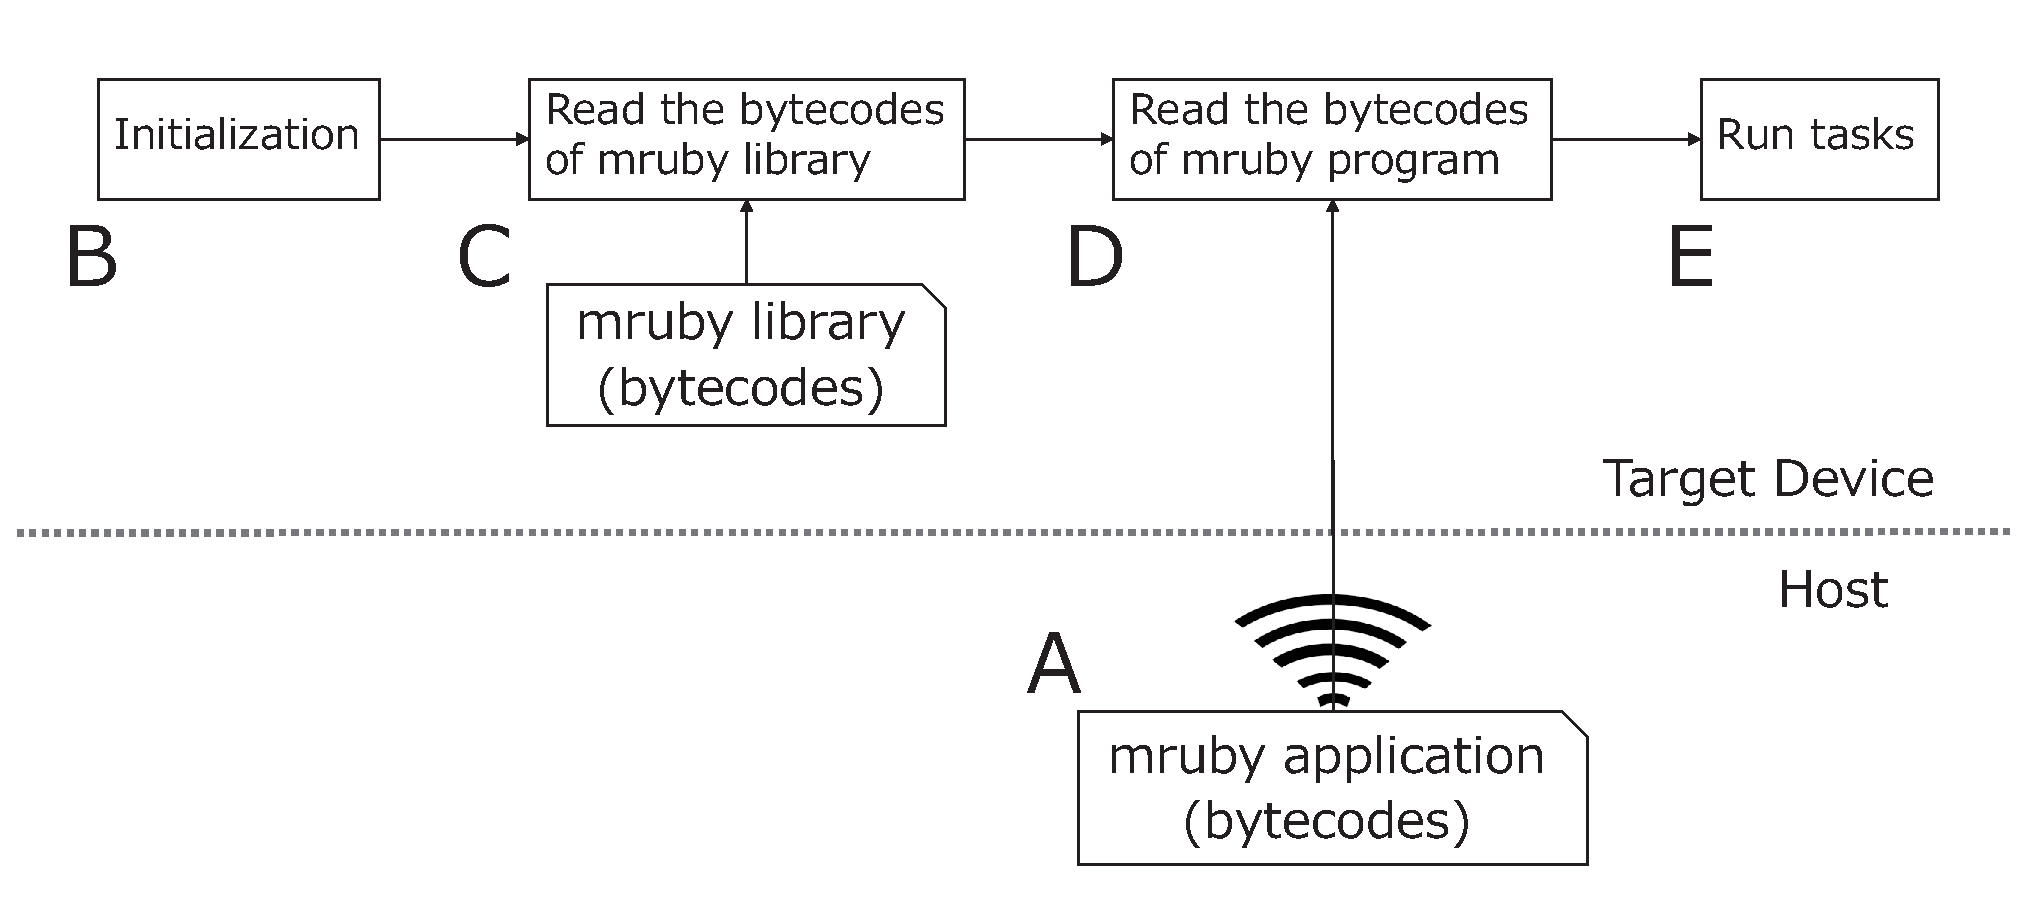
\includegraphics[width=8cm,clip]{figure/control_flow.eps}
    \vspace{1mm}
\caption{Process Flow of \DIFaddbeginFL \DIFaddFL{Bluetooth loader for }\DIFaddendFL mruby bytecode\DIFdelbeginFL \DIFdelFL{loader using Bluetooth}\DIFdelendFL }
    \vspace{1mm}
\label{fig:control_flow}
\end{figure}

\begin{figure}[t]
\centering
\begin{lstlisting}
/* tRiteVMBluetooth.cdl */
celltype \DIFdelbeginFL \DIFdelFL{tRiteVMBluetooth}\DIFdelendFL \DIFaddbeginFL \DIFaddFL{tRiteVMBluetooth1 }\DIFaddendFL {
    entry sTaskBody eMrubyBody;
    [optional] call sEventflag cEventflag[];
    [optional] call sSemaphore cSemaphore;
    attr {
      [omit]char_t *mrubyLib;
      char_t *irepLib = 
                    C_EXP("&$cell_global$_irep");
      uint32_t irepAppSize = 
                    C_EXP( BUFFER_SIZE );
      FLGPTN setptn;
    };
    var {
        mrb_state *mrb;
        mrbc_context *context;
        [size_is(irepAppSize)] uint8_t *irepApp;
    };
};
\end{lstlisting}
\vspace{1mm}
\caption{Celltype Description for RiteVM with \DIFaddbeginFL \DIFaddFL{Bluetooth loader for }\DIFaddendFL mruby bytecode\DIFdelbeginFL \DIFdelFL{loader using Bluetooth}\DIFdelendFL }
\vspace{1mm}
\label{celltype_mrubybluetooth}
\end{figure}

\begin{figure}[t]
\centering
\begin{lstlisting}
/* tRiteVMBluetooth.c */
void
eMrubyBody_main( CELLIDX idx )
{
  /* Omit: start of exclusive process by semaphore */
  /* Receive the bytecode via Bluetooth */
  bluetooth_loader( VAR_irepApp );
  /* Omit: end of exclusive process by semaphore */
  /* New interpreter instance */
  VAR_mrb = mrb_open();
  /* Omit: error check for mrb_state */
  /* New mruby context */
  VAR_context = mrbc_context_new( VAR_mrb );
  /* Omit: initialization of mruby-TECS bridge */
  /* Omit: synchronization of
                starting mruby application */
  /* Load mruby library bytecode */
  mrb_load_irep_cxt( VAR_mrb,
                        ATTR_irepLib, VAR_context );
  /* Load mruby application bytecode and run */
  mrb_load_irep_cxt( VAR_mrb,
                        VAR_irepApp, VAR_context );
  if ( mrb->exc ) {
    /* Failure to execute */
    mrb_p( VAR_mrb, 
                mrb_obj_value( VAR_mrb->exc ) );
    exit( 0 );
  }
  /* Omit: synchronization of
                finishing mruby application */
  /* Free mruby context */
  mrbc_context_free( VAR_mrb, VAR_context );
  /* Free interpreter instance */
  mrb_close( VAR_mrb );
}

\end{lstlisting}
\vspace{1mm}
\caption{Main code for RiteVM with \DIFaddbeginFL \DIFaddFL{Bluetooth loader for }\DIFaddendFL mruby bytecode\DIFdelbeginFL \DIFdelFL{loader using Bluetooth}\DIFdelendFL }
\vspace{1mm}
\label{maincode_mrubybluetooth}
\end{figure}

Figure \ref{fig:control_flow} shows the process flow of executing mruby program in the component of RiteVM with \DIFdelbegin \DIFdel{mruby bytecode loader using Bluetooth }\DIFdelend \DIFaddbegin \DIFadd{Bluetooth loader for mruby bytecode }\DIFaddend such as RiteVMBluetooth1.
The concrete main code of tRiteVMBluetooth is shown in Figure \ref{maincode_mrubybluetooth}.

First, the \DIFdelbegin \DIFdel{mruby bytecode }\DIFdelend \DIFaddbegin \DIFadd{Bluetooth }\DIFaddend loader receives the mruby application bytecode transferred from the host (Figure \ref{fig:control_flow}:A, Lines 6-7 in Figure \ref{maincode_mrubybluetooth}).
The bytecode is stored in the component variable such as VAR\_irepApp shown in Figure \ref{celltype_mrubybluetooth}.
This process is exclusively carried out by the semaphore.

Second, pointers of {\myit mrb\_state} and {\myit mrbc\_context}, and mruby-TECS bridges are initialized (Figure \ref{fig:control_flow}:B, Lines 9-14 in Figure \ref{maincode_mrubybluetooth}).
{\myit VAR\_mrb} and {\myit VAR\_context} shows the variable of the {\myit cell}.
{\myit mrb\_state} is a set of states and global variables used in mruby.
Synchronization of multiple tasks is performed in this processing phase.
The RiteVM that ended up here waits for the other RiteVM to finish loading and initialization.

Third, the RiteVM reads the bytecode of mruby libraries (Figure \ref{fig:control_flow}:C, Lines 17-19 in Figure \ref{maincode_mrubybluetooth}).
mruby libraries are a set of Ruby classes such as motor class and sensor class.
For example, motor class defines methods to rotate and stop a motor.
The tRiteVMBluetooth {\myit cell} has attributes as shown in Figure \ref{celltype_mrubybluetooth}.
{\myit ATTR} shows the attribute, which is a fixed value and not rewritten unlike {\myit VAR}.
The {\myit mrubyLib} indicates the program files of mruby libraries.
{\myit mrubyLib} is the attribute because mruby libraries are not modified in the proposed development process.
{\myit [omit]} is only used for the TECS generator, thus the attribute, {\myit mrubyLib}, does not consume memory.
The {\myit irepLib} is the pointer of the array stored the bytecode of mruby libraries.
In short, the bytecode of mruby libraries is stored as an attribute of the component when compiling for the first time.

Fourth, the RiteVM reads the bytecode of the mruby application transferred with Bluetooth (Figure \ref{fig:control_flow}:D, Lines 20-22 in Figure \ref{maincode_mrubybluetooth}).
The mruby application bytecode is stored in an array of {\myit irepApp}.
The array is different from that of holding the mruby library bytecode.
Two bytecodes are read separately in the RiteVM.

Finally, the mruby task runs (Figure \ref{fig:control_flow}:E, \DIFdelbegin \DIFdel{Figure \ref{maincode_mrubybluetooth}:}\DIFdelend \DIFaddbegin \DIFadd{Lines }\DIFaddend 20-22 \DIFaddbegin \DIFadd{in Figure \ref{maincode_mrubybluetooth}}\DIFaddend ).
When the mruby application is modified, only the bytecode of the modified application should be transferred.
mruby libraries need not be touched because libraries are not normally changed.

The process shown in Figure \ref{maincode_mrubybluetooth}:23-28 is carried out when an exception occurs.
When all mruby applications finish, mrb\_state and mrbc\_context are freed (Figure \ref{maincode_mrubybluetooth}:31-34).
The proposed framework supports continuous loading, thus this process loops.
After freeing variables, RiteVM will become the state to wait for the next mruby application bytecode.
\subsection{RiteVM Scheduler}
\label{sec:RiteVM Scheduler}
This section describes implementation of RiteVM scheduler in the proposed framework.
mruby on TECS has supported multitasking.
However, multitask processing in mruby on TECS requires the knowledge of the RTOS (TOPPERS/HRP2) for developers.

One of approaches for multitasking is co-routine.
Co-routine is a cooperative thread, and scheduled by developers with the functions such as {\myit resume} and {\myit yield}. 
(Ruby co-routine is defined in class Fiber \cite{url:co-routine})
Co-routine is a non-preemptive multitasking, and does not receive the OS's support because developers have to switch tasks manually.
Co-routine can not take advantage of multi core processing.

Besides, as another method, {\myit delay()}, a service call of $\mu$ITRON, can be used for multitasking.
This service call delays the execution of the own task for the time of the argument.
%In the approach of {\myit delay} function, developers have to schedule as the same as co-routine.
{\myit delay()} is needed when scheduling fixed-priority tasks.
However, the programming applied to {\myit delay()} is difficult to use in the case of fair scheduling.

As an approach for multitask processing, the proposed framework provides the RiteVM scheduler which is a fair scheduler and runs multiple tasks equally.
The RiteVM scheduler is utilized only when application tasks have the same priority.
mruby applications can run in concurrent without developers calling the OS's function.
The application programs can also utilize the existing programs since the structures of the programs are not changed. 

The RiteVM scheduler is a fair scheduler and implemented as a TECS component in the proposed framework.
Therefore, when developers create software in priority-based scheduling, the RiteVM scheduler can be easily removed.
\DIFaddbegin 

\DIFaddend \subsubsection{Design of RiteVM Scheduler}
A RiteVM scheduler is a periodic handler \DIFdelbegin \DIFdel{, and calls }\DIFdelend \DIFaddbegin \DIFadd{and }\DIFaddend {\myit rotateReadyQueue}, a service call of $\mu$ITRON to switch tasks with the same priority\DIFaddbegin \DIFadd{, is implemented as the main process of the handler}\DIFaddend .
In other words, the RiteVM scheduler calls {\myit rotateReadyQueue} cyclically.
The design of the RiteVM scheduler is shown in Figure \ref{fig:rotateReadyQueue}. 
{\myit rotateReadyQueue} is described as follows.

The case is assumed that there are two tasks with the same priority, and both tasks are in an infinite loop.
In the current system, when one task is executed first, another task would not be executed.
That is because the task with first execution runs in the loop.

When {\myit rotateReadyQueue} is called, tasks with the same priority are switched as shown in Figure \ref{fig:rotateReadyQueue}.
The argument of {\myit rotateReadyQueue} is the priority.

\DIFdelbegin \DIFdel{The }\DIFdelend {\myit rotateReadyQueue} can be performed if the number of tasks is more than two.
For example, three tasks are in the order: \DIFdelbegin \DIFdel{task 1, 2, and3.
}\DIFdelend \DIFaddbegin \DIFadd{task1, task2, and, task3.
}\DIFaddend In this case, the order is rotated, \DIFdelbegin \DIFdel{task 2, 3 and, 1}\DIFdelend \DIFaddbegin \DIFadd{task2, task3, and, task1}\DIFaddend , when the {\myit rotateReadyQueue} is called.

\begin{figure}[t]
    \centering
    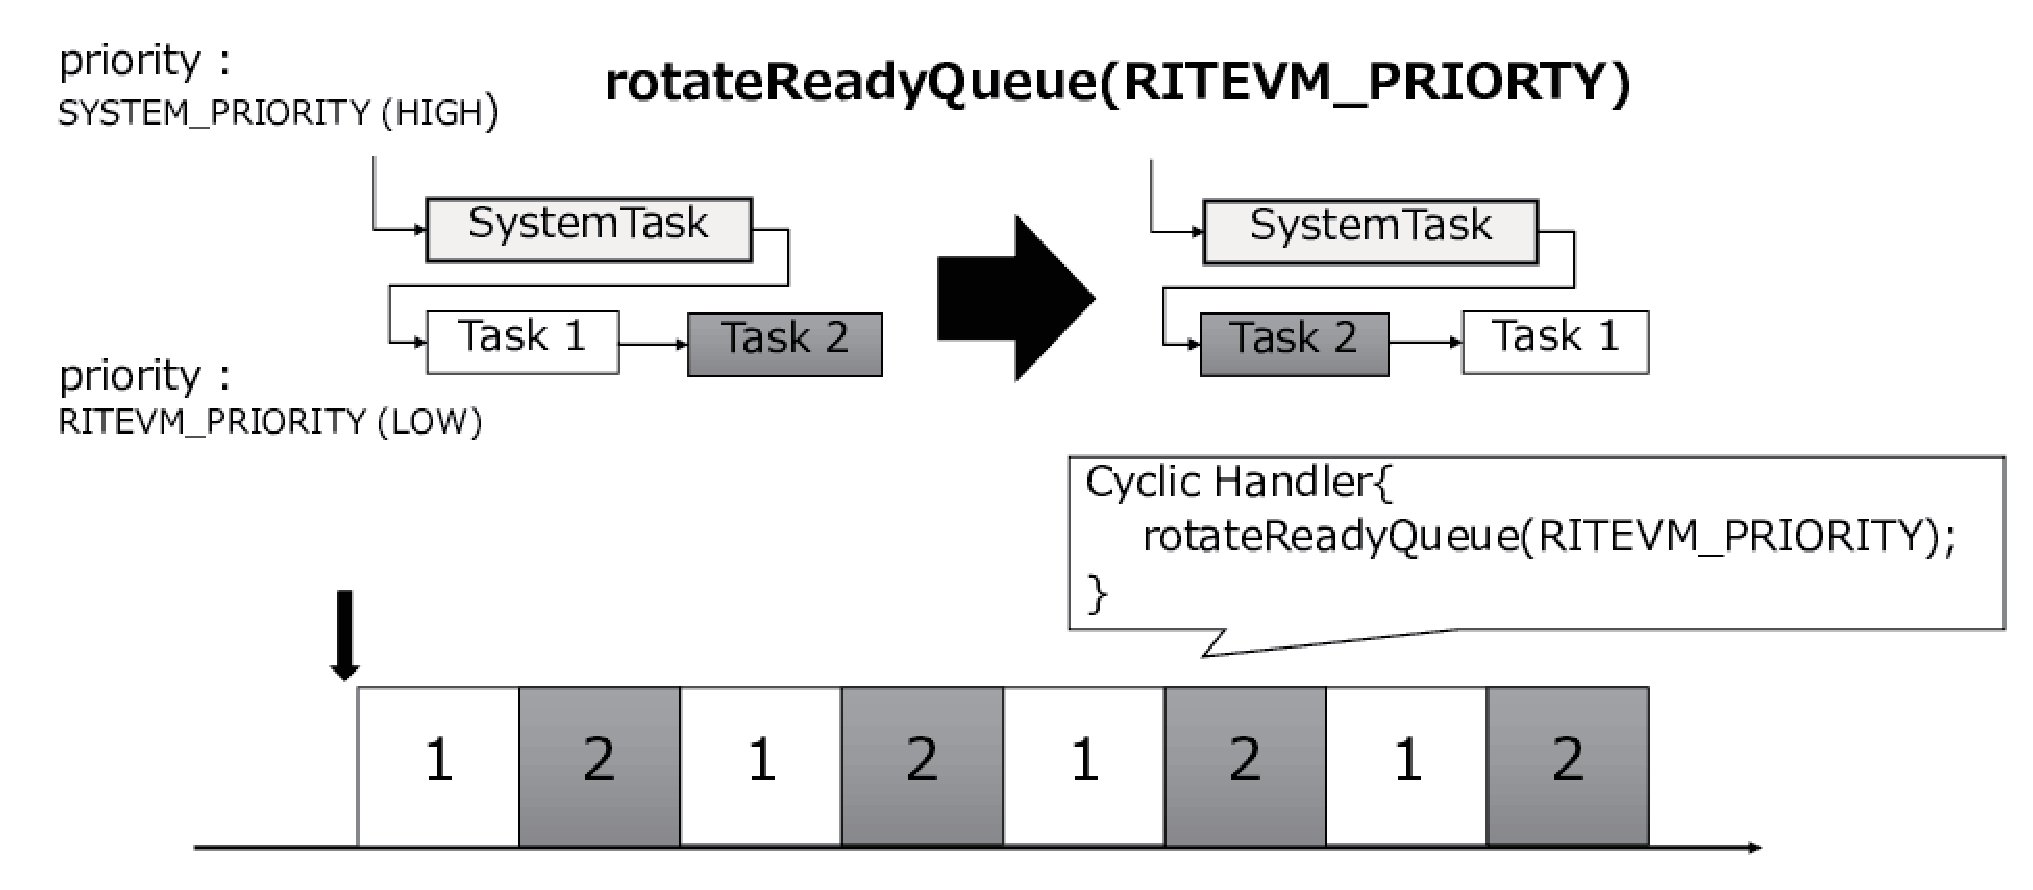
\includegraphics[width=8cm,clip]{figure/rotateReadyQueue.eps}
    \vspace{1mm}
\caption{The design of RiteVM scheduler}
    \vspace{1mm}
\label{fig:rotateReadyQueue}
\end{figure} 

\subsubsection{Component of RiteVM Scheduler}
Figure \ref{fig:cyclic_handler} shows the component diagram of RiteVM scheduler.
The component of RiteVM scheduler consist of CyclicHandler and RiteVMSchedulerMain.
CyclicHandler {\myit cell} configures the periodic handler based on $\mu$ITRON.
\DIFdelbegin \DIFdel{Cyclic }\DIFdelend %DIF > Cyclic handlers based on $\mu$ITRON are described in detail \cite{par:microITRON}.
\DIFaddbegin \DIFadd{\mbox{%DIFAUXCMD
\cite{par:microITRON} }%DIFAUXCMD
describes cyclic }\DIFaddend handlers based on $\mu$ITRON \DIFdelbegin \DIFdel{are described in detail\mbox{%DIFAUXCMD
\cite{par:microITRON}}%DIFAUXCMD
}\DIFdelend \DIFaddbegin \DIFadd{in detail}\DIFaddend .
CyclicHandler {\myit cell} has attributes of the {\myit cell}.
RiteVMSchedulerMain {\myit cell} is a component to perform the processing body of a periodic handler.
{\myit rotateReadyQueue} is implemented as the body.
Figure \ref{celltype_cyclic_handler} shows tRiteVMScheduler {\myit celltype}, which is the {\myit composite cell} consisting of two {\myit cell}s.
The {\myit call} port of RiteVMSchedulerMain is connected with the {\myit entry} port of the Kernel {\myit cell} ({\myit tKernel.eiKernel}) to call functions of the kernel. 
The attribute is used as an arguments of {\myit rotateReadyQueue}.

Figure \ref{build_cyclic_handler} shows the build description of RiteVM scheduler.
RiteVMScheduler {\myit cell} has attributes to configure the scheduler such as attribute, cyclicTime, cyclicPhase, and priority.
In this case, RiteVM scheduler is executed when it is generated because the attribute is {\myit TA\_STA} that represents the periodic handler is in an operational state after the creation.
The scheduler executes every one msec.
RITEVM\_PRIORITY defines the priority of mruby tasks.
In the main of CyclicMain, {\myit rotateReadyQueue} is implemented and the priority is passed as the argument.

\begin{figure}[t]
    \centering
    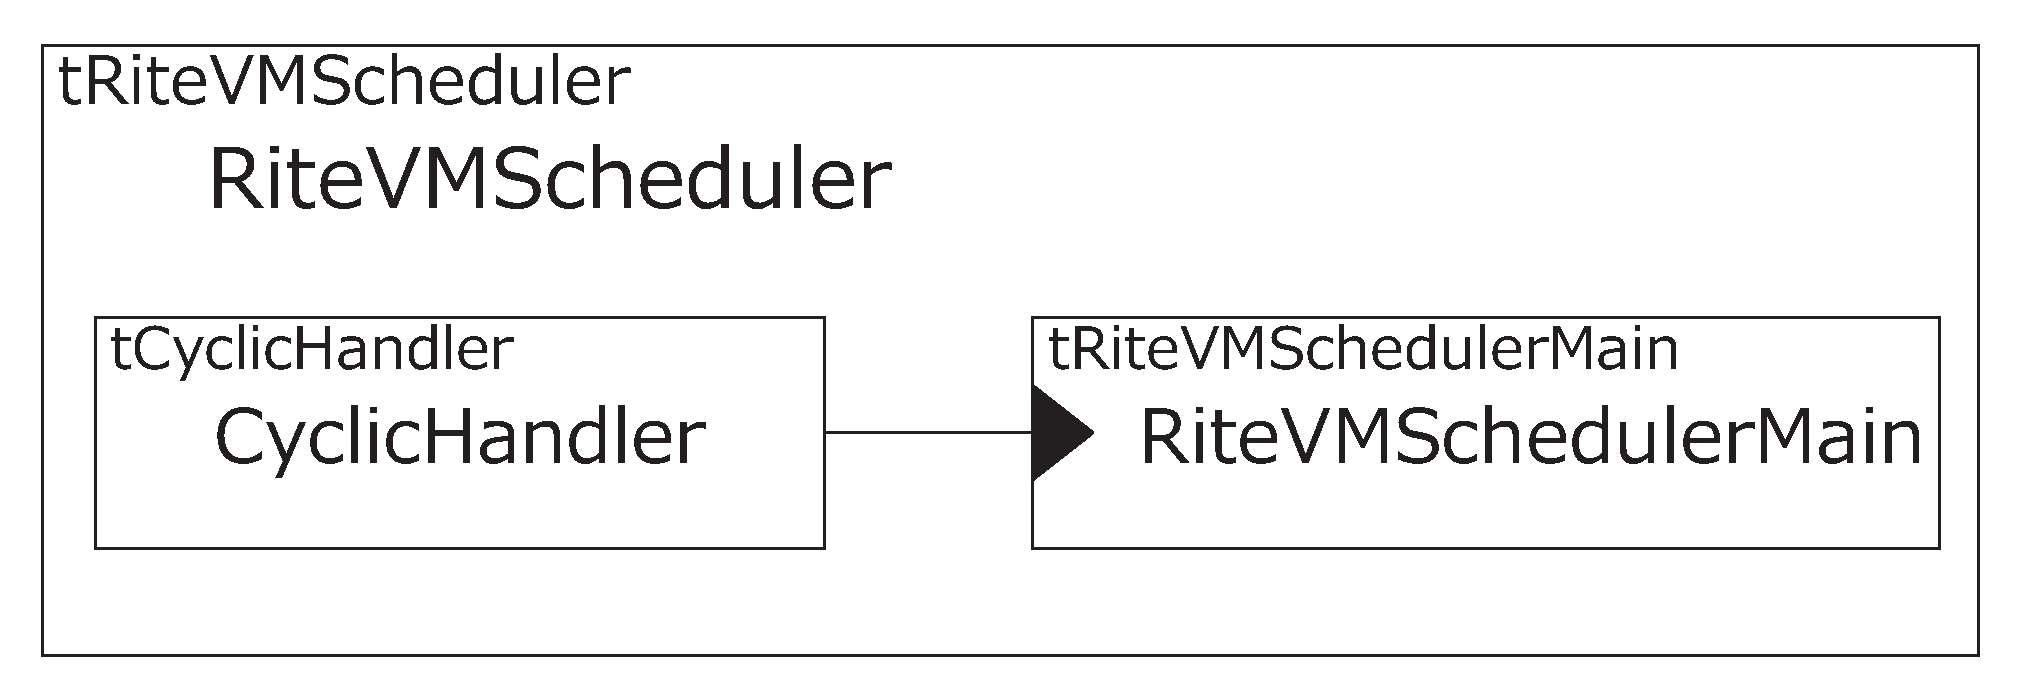
\includegraphics[width=8cm,clip]{figure/cyclic_handler.eps}
    \vspace{1mm}
\caption{Component Diagram of RiteVM Scheduler}
    \vspace{1mm}
\label{fig:cyclic_handler}
\end{figure}
\begin{figure}[t]
    \centering
    \begin{lstlisting}
/* tRiteVMScheduler.cdl */
celltype tCyclicHandler {
    [inline] entry sCyclic eCyclic;
    call siHandlerBody  ciBody;
    attr {
        [omit] ATR    attribute   = C_EXP("TA_NULL");
    	[omit] RELTIM cyclicTime;
    	[omit] RELTIM cyclicPhase;
    };
};
celltype tRiteVMSchedulerMain {
    require tKernel.eiKernel;
    entry   siHandlerBody eiBody;
    attr {
        PRI priority;
    };
};

composite tRiteVMScheduler {
    attr {
        ATR    attribute      = C_EXP("TA_NULL");
        RELTIM cyclicTime  = 1;
        RELTIM cyclicPhase = 1;
        PRI    priority;
    };
    cell tRiteVMSchedulerMain RiteVMSchedulerMain {
        priority = composite.priority;
    };
    cell tCyclicHandler CyclicHandler {
        ciBody      = RiteVMSchedulerMain.eiBody;
        attribute   = composite.attribute;
        cyclicTime  = composite.cyclicTime;
        cyclicPhase = composite.cyclicPhase;
    };
};
    \end{lstlisting}
    \vspace{1mm}
\caption{Celltype Description of RiteVM Scheduler}
    \vspace{1mm}
\label{celltype_cyclic_handler}
\end{figure}
\begin{figure}[t]
    \centering
    \begin{lstlisting}
cell tRiteVMScheduler RiteVMScheduler {
    attribute   = C_EXP("TA_STA");
    cyclicTime  = 1;
    cyclicPhase = 1;
    priority    =
        C_EXP("RITEVM_PRIORITY");
};
\end{lstlisting}
    \vspace{1mm}
\caption{Build Description of \DIFdelbeginFL \DIFdelFL{RiteV }\DIFdelendFL \DIFaddbeginFL \DIFaddFL{RiteVM }\DIFaddendFL Scheduler}
    \vspace{1mm}
\label{build_cyclic_handler}
\end{figure}

\subsection{Synchronization of Multiple RiteVM Tasks}
In the proposed framework, RiteVMs read mruby bytecodes, and then execute the applications.
Eventflag, one of synchronous processing, is applied to synchronize the starting of multiple mruby applications.
Each task sets the flag pattern such as 0x01 (01) and 0x02 (10), and then waits the flag pattern, 0x3 (11), with AND.
This process can also apply to the case of the more tasks.
For example, in the case of the four RiteVM tasks, each task sets the flag pattern such as 0x01 (0001), 0x02 (0010), 0x04 (0100)  and 0x08 (1000), and then waits 0x0f (1111) with AND as shown in Figure \ref{fig:Eventflag} (A).

In addition, the end of mruby applications is synchronized to accept the continuous loading.
The ending synchronization prevents a RiteVM whose application immediately finishes from waiting the next loading.
All of mruby applications finish at the same time, and all RiteVMs wait for receiving the next mruby application bytecodes. 

\begin{figure}[t]
    \centering
    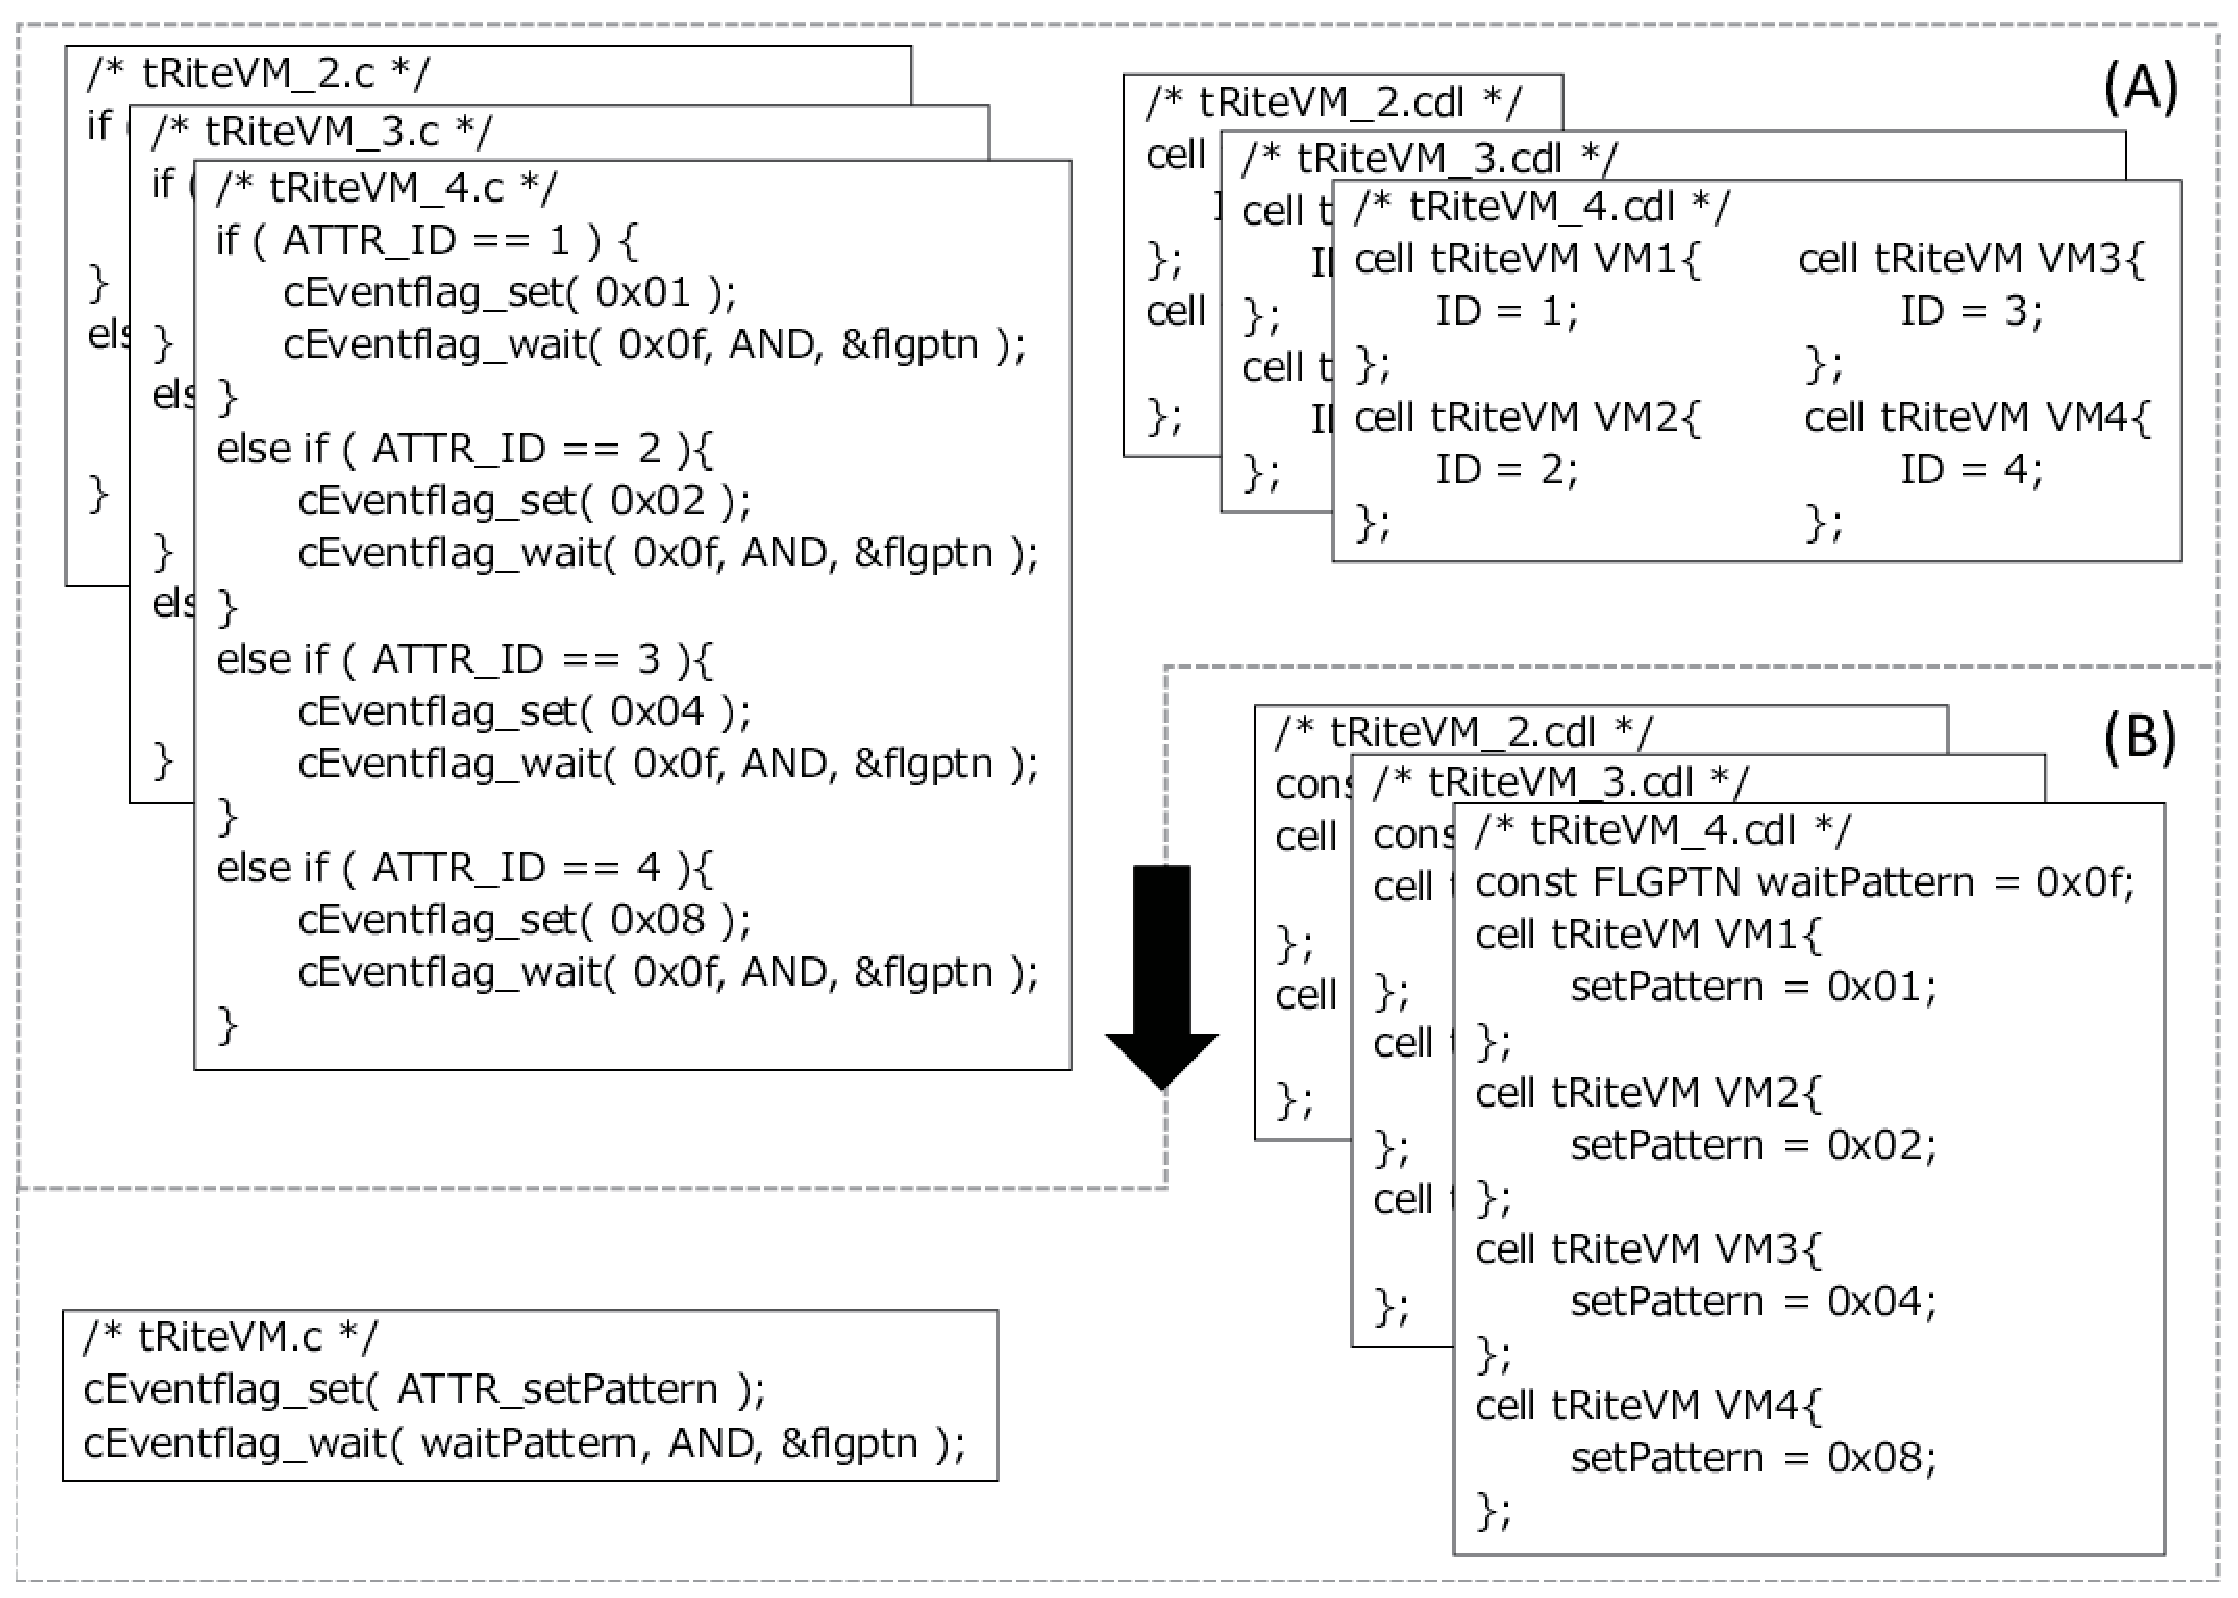
\includegraphics[width=8cm,clip]{figure/Eventflag.eps}
    \vspace{1mm}
\caption{The design for Eventflag using TECS (only differences)}
    \vspace{1mm}
\label{fig:Eventflag}
\end{figure}

\subsection{Utilization of Component-Based Development}
This section describes the design applying component-based development.

In the framework, RiteVMs, the RiteVM scheduler, and Eventflag are implemented as components.
Therefore, developers can easily add or remove these components and also reuse them.
For example, if RiteVM scheduler is not necessary for software, developers should only comment out the \DIFdelbegin \DIFdel{.cdl }\DIFdelend \DIFaddbegin \DIFadd{CDL }\DIFaddend file such as {\myit //import(<tRiteVMScheduler.cdl>);}.
This advantage of CBD saves developers the labor of rewriting a kernel configuration file.

In addition, the code size can decrease by developing with component-based. 
In the proposed framework, the advantage is applied in the Eventflag component.
The set pattern and wait pattern are defined as attributes of the component as shown in Figure \ref{fig:Eventflag} (B).
This design such as {\myit cEventflag\_set(ATTR\_setPattern)} enables the program without ``if" statements and reuses the identical \DIFdelbegin \DIFdel{.c }\DIFdelend \DIFaddbegin \DIFadd{C }\DIFaddend file.
Developers do not need to modify the \DIFdelbegin \DIFdel{.c }\DIFdelend \DIFaddbegin \DIFadd{C }\DIFaddend file because the \DIFdelbegin \DIFdel{.cdl }\DIFdelend \DIFaddbegin \DIFadd{CDL }\DIFaddend files are prepared in accordance with the number of RiteVMs\DIFaddbegin \DIFadd{.
}\DIFaddend In addition, the components of Eventflag are built with {\myit [optional]} in TECS.
{\myit [optional]} means that the codes are run only when the call port is connected.
The \DIFdelbegin \DIFdel{.c }\DIFdelend \DIFaddbegin \DIFadd{C }\DIFaddend file does not be rewritten even if developers do not use Eventflag. 

\section{Experimental Evaluation}
\label{sec:Evaluation}
This section mentions experimental results and their consideration.
To analyze the advantages of the proposed framework, the evaluations are performed as follows.
\begin{itemize}
%    \item Execution time of the platform
    \item Size and time for transferred mruby bytecodes
    \item Execution time with singletasking, co-routine, and proposed multitasking
    \item Overhead for periodic time
    \item Synchronization of multiple RiteVM tasks
    \item Code size utilizing component-based development 
\end{itemize}

These evaluations are performed in order to indicate that \DIFdelbegin \DIFdel{an mruby bytecode }\DIFdelend \DIFaddbegin \DIFadd{a Bluetooth }\DIFaddend loader improves the software development efficiency, and that the proposed multitask processing effectively executes compared with singletasking or co-routine, and also the overhead of the cyclic period.
This paper demonstrates the proposed system on a LEGO MINDSTORMS EV3 \cite{par:EV3} (300MHz ARM9-based Sitara AM1808 system-on-a-chip) compiled with gcc 4.9.3 -O2 and mruby version 1.2.0.

\subsection{Improving the software development efficiency by \DIFdelbegin \DIFdel{mruby bytecode }\DIFdelend \DIFaddbegin \DIFadd{Bluetooth }\DIFaddend loader}
The \DIFdelbegin \DIFdel{mruby bytecode loader using Bluetooth }\DIFdelend \DIFaddbegin \DIFadd{Bluetooth loader for mruby bytecode }\DIFaddend can save time to develop software.
In the proposed framework, developers do not need to rewrite a storage/ROM device because the bytecode should be just transferred.
For example, when mruby programs are modified, developers must pull out an SD card from the target device, connect the host PC, compile/link the platform, and insert the SD card in the target device, in the experimental environment such as LEGO MINDSTORMS EV3.
In addtion, it can save the time to restart a target \DIFdelbegin \DIFdel{OS.
}\subsubsection{\DIFdel{Size and time for transferred mruby bytecodes}}
%DIFAUXCMD
\addtocounter{subsubsection}{-1}%DIFAUXCMD
\DIFdelend \DIFaddbegin \DIFadd{RTOS.
}

%DIF > \subsubsection{Size and time for transferred mruby bytecodes}
\DIFaddend In the framework, to further improve the software development efficiency, developers transfers only the mruby application bytecode and mruby libraries are incorporated in the platform.
The size, load process time, and compilation time for mruby application and mruby application including library is shown in Table \ref{tab:size_and_time}.
The overhead of load processing is 50.933 msec, which it takes to load a zero bytes bytecode.
Similarly, the overhead of compilation is 46.9 msec, which it takes to compile a zero bytes program.
The mruby application bytecode is smaller and faster than that of including mruby libraries in all terms.
The difference becomes larger as the number of RiteVMs increases because it takes the 50 msec overhead per one RiteVM. 
%In the proposed framework, developers send only mruby application and prepare mruby library in advance.
%Therefore, the design can send the bytecode faster.
%In addition, the design can save the time to rewrite a storage/ROM device, and to restart an OS.
These advantages lead improvement of the software development efficiency.

\begin{table}[t]
    \centering
    \vspace{1mm}
\caption{Comparison of the size and load process time between an mruby application including mruby libraries and not}
    \vspace{1mm}
    %\scriptsize
    {\tabcolsep=0.1cm
    \begin{tabular}{c||c|c|c}
                            & App\&Lib     & App        &   App\&Lib/App  \\ \hline
          Bytecode Size     & 14,044 bytes & 199 bytes  &   $\times$70.6          \\ %\hline
          Loading Time      & 305.081 msec & 7.774 msec &   $\times$39.2          \\
          Compile Time  & 8.7 msec     & 0.3 msec   &   $\times$29.0          \\
    \end{tabular}
    }
    \label{tab:size_and_time}
\end{table}

\subsection{RiteVM Scheduler}
The comparison of the application execution time with singletasking, co-routine, and multitasking is shown in Figure \ref{fig:comparison_s_c_m}.
The 100,000 times loop program is used as mruby application for evaluation of execution time.
In detail, the singletask program loops 100,000 times, and the multitask and co-routine programs loop 50,000 times in each task.
\DIFdelbegin \subsubsection{\DIFdel{Execution time with singletasking, co-routine, and purposed multitasking}}
%DIFAUXCMD
\addtocounter{subsubsection}{-1}%DIFAUXCMD
\DIFdelend \DIFaddbegin 

%DIF > \subsubsection{Execution time with singletasking, co-routine, and purposed multitasking}
\DIFaddend In Figure \ref{fig:comparison_s_c_m}, the periodic time of the periodic handler for multitasking is one msec.
%While multitask's execution time is slower than singletask's, co-routine takes more time than multitask to execute an mruby application.
This result shows the proposed design is superior to co-routine in terms of execution time.
Moreover, developers can utilize the scheduler practically because the overhead of the RiteVM scheduler is about 5 \%.
The scheduler interrupts and switches tasks, which causes this overhead.
It takes about three $\mu$sec on average to switch tasks once.
%The number of switching tasks is from 500 to 600 because singletasking process in Figure \ref{fig:comparison_s_c_m} takes about 540 msec.
%Therefore, the overhead of multitasking is 0.5 \% or less, and multitasking can be used without the overhead.

\begin{figure}[t]
    \centering
    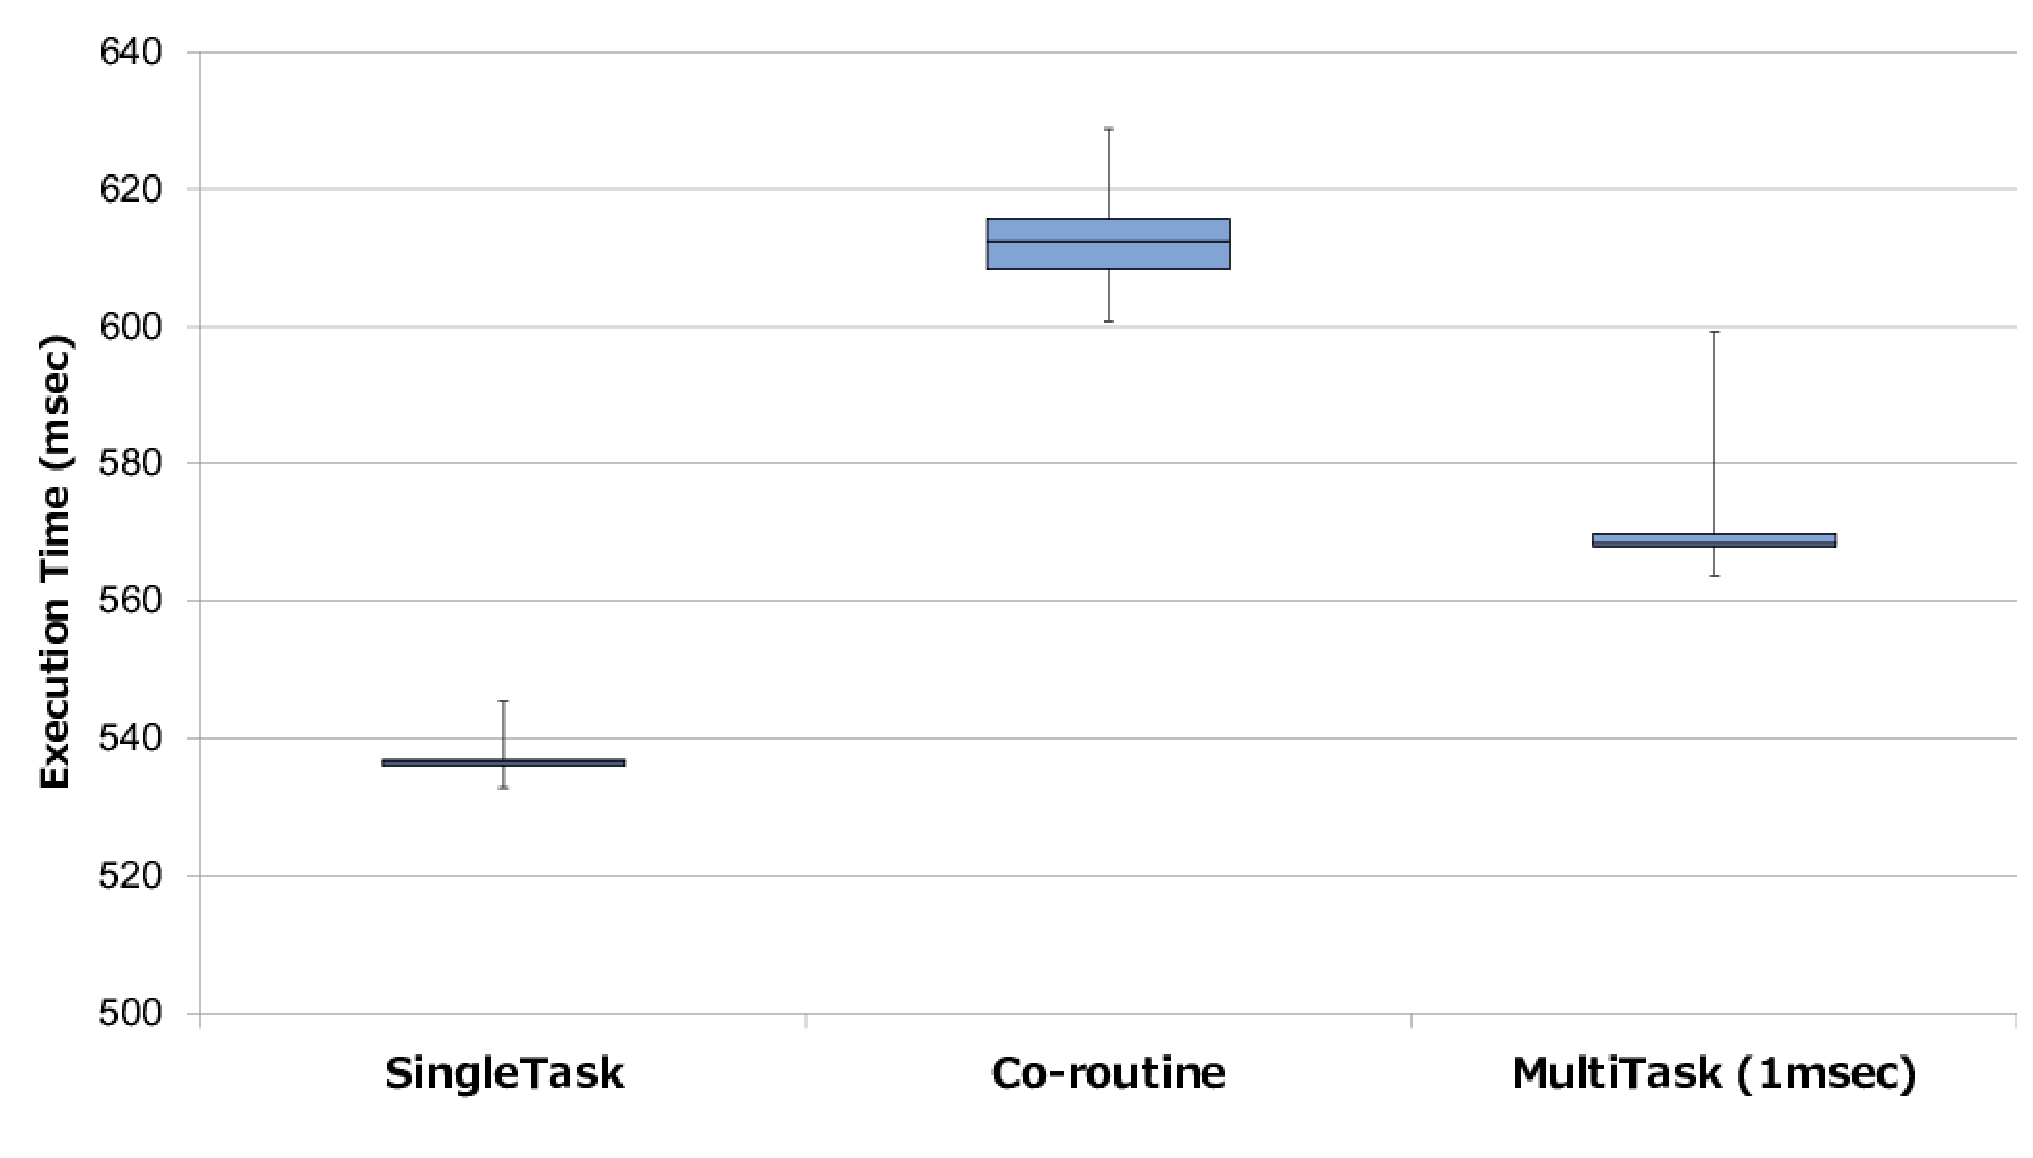
\includegraphics[width=8cm,clip]{figure/comparison_s_c_m.eps}
    \vspace{1mm}
\caption{Comparison of the application execution time with singletask, co-routine, and multitask}
    \vspace{1mm}
\label{fig:comparison_s_c_m}
\end{figure}

\DIFdelbegin \subsubsection{\DIFdel{Overhead for periodic time}}
%DIFAUXCMD
\addtocounter{subsubsection}{-1}%DIFAUXCMD
\DIFdelend %DIF > \subsubsection{Overhead for periodic time}
Figure \ref{fig:comparison_msec} shows the execution time of multitasking with the periodic handler.
A lower limit of the periodic time is one msec due to the specification of TOPPERS/HRP2, the used RTOS.
More than eight msec do not be evaluated in this paper because it is thought the larger periodic time influences applications.
%Each execution time of cyclic period is the same as the others.
%That is because the overhead of switching tasks (about 3 $\mu$sec) is small in comparison with the execution time.
The execution time decreases as the periodic time become larger, because the number of switching tasks decreases.
The execution time of one msec is only about 1 \% lager than that of eight msec.
The RiteVM scheduler with small periodic time can effectively execute multiple tasks because the periodic time overhead is not large.
%This results also shows the overhead becomes smaller as the periodic time is larger, because the overhead depends on the number of switching tasks.
The smaller periodic time is better in multitasking due to concurrent and/or parallel processing.

\begin{figure}[t]
    \centering
    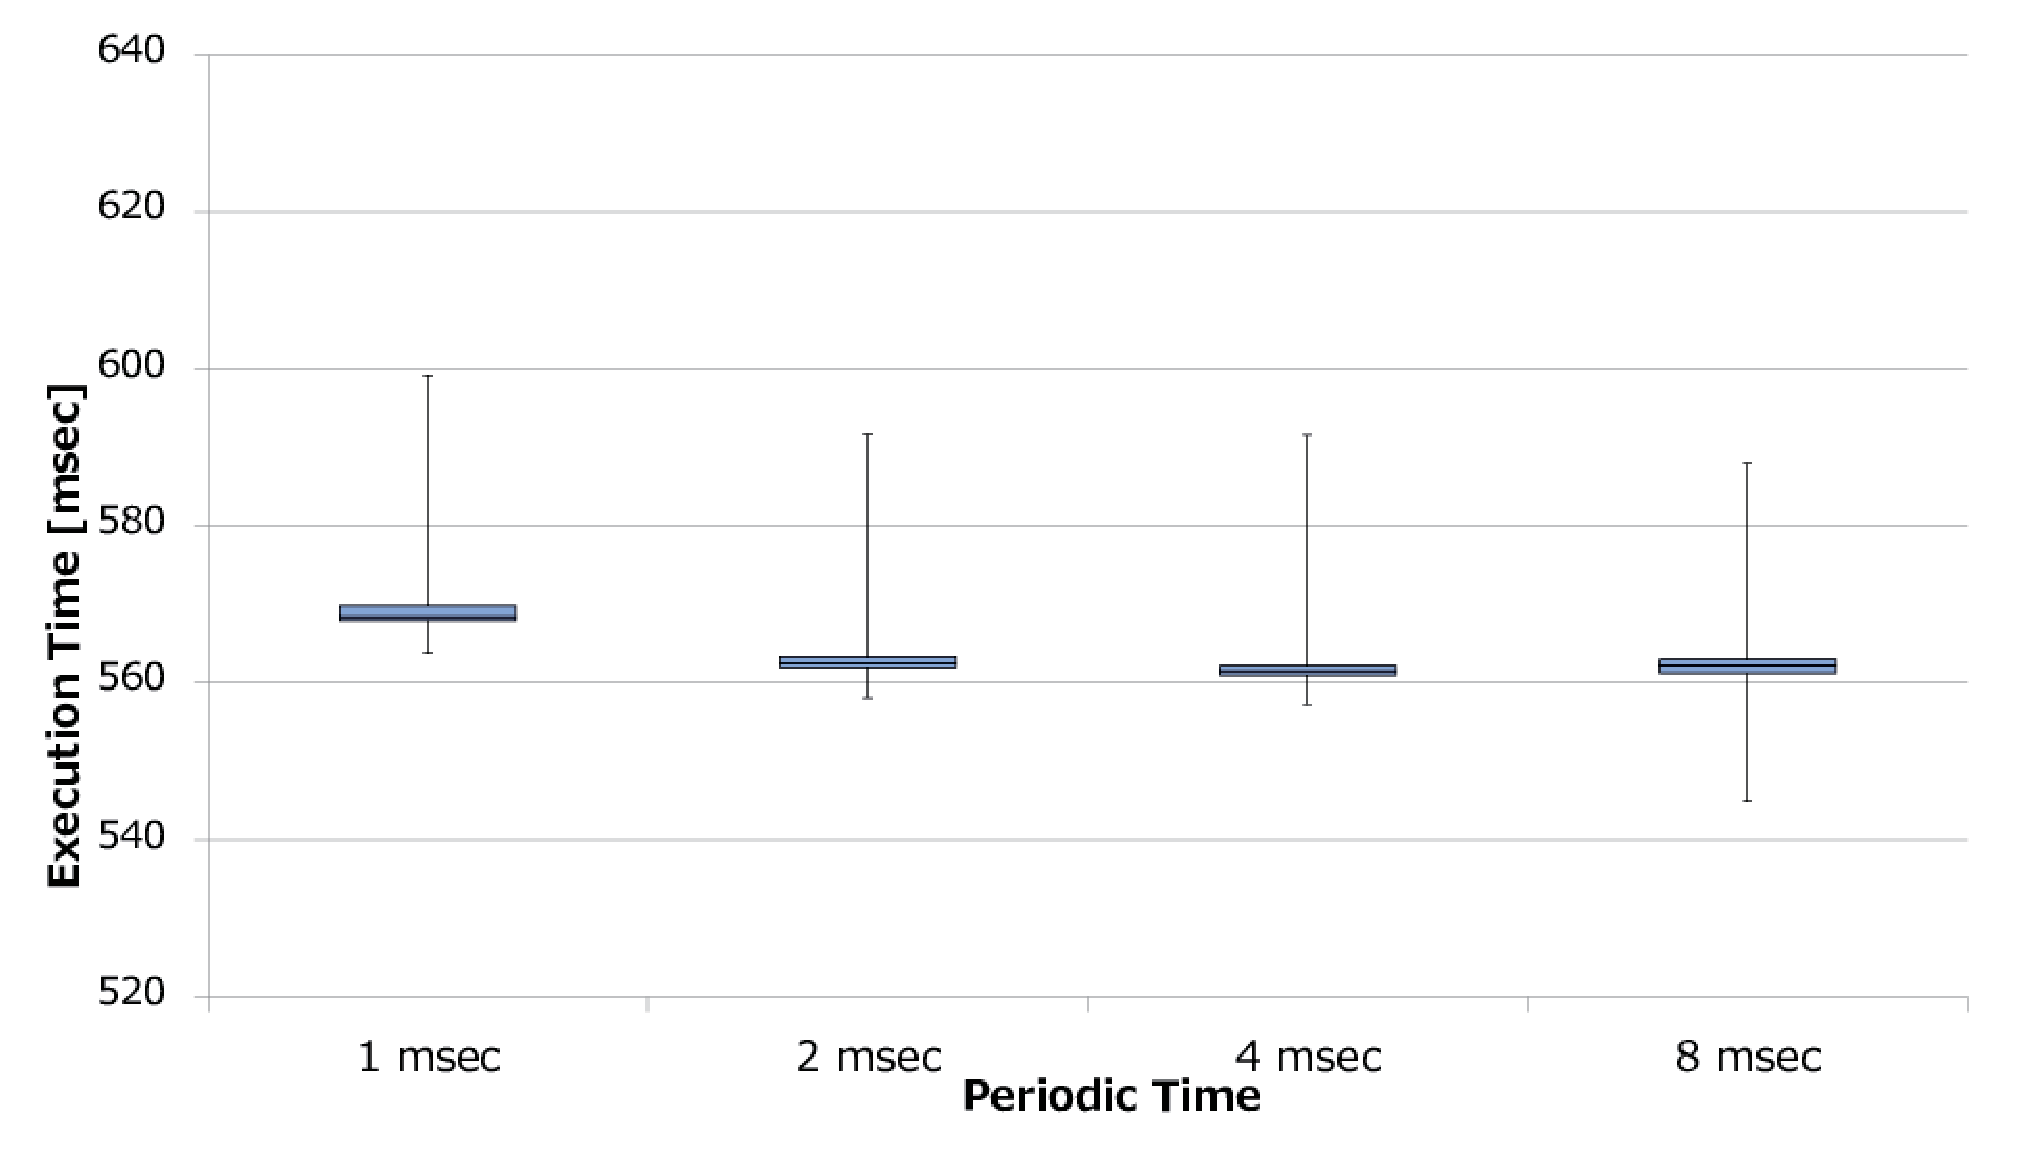
\includegraphics[width=8cm,clip]{figure/comparison_msec.eps}
    \vspace{1mm}
\caption{Comparison of the overhead for each cyclic period of RiteVM scheduler}
    \vspace{1mm}
\label{fig:comparison_msec}
\end{figure}

\subsection{Synchronization of multiple RiteVM tasks}
To execute mulitiple mruby applications, synchronization mechanism of RiteVM tasks is supported in the proposed framework.
We measured the time from first RiteVM task executing to last RiteVM task executing, and confirm that the time is within (periodic time)$\times$(the number of RiteVM tasks $-$ 1).
Figure \ref{fig:eval_synchronization} shows the case of four RiteVM tasks.
The periodic time is one msec, and the number of RiteVM is four.
The time is within three msec as shown in Figure \ref{fig:eval_synchronization}, which shows synchronization of multiple RiteVM tasks is performed.

\begin{figure}[t]
    \centering
    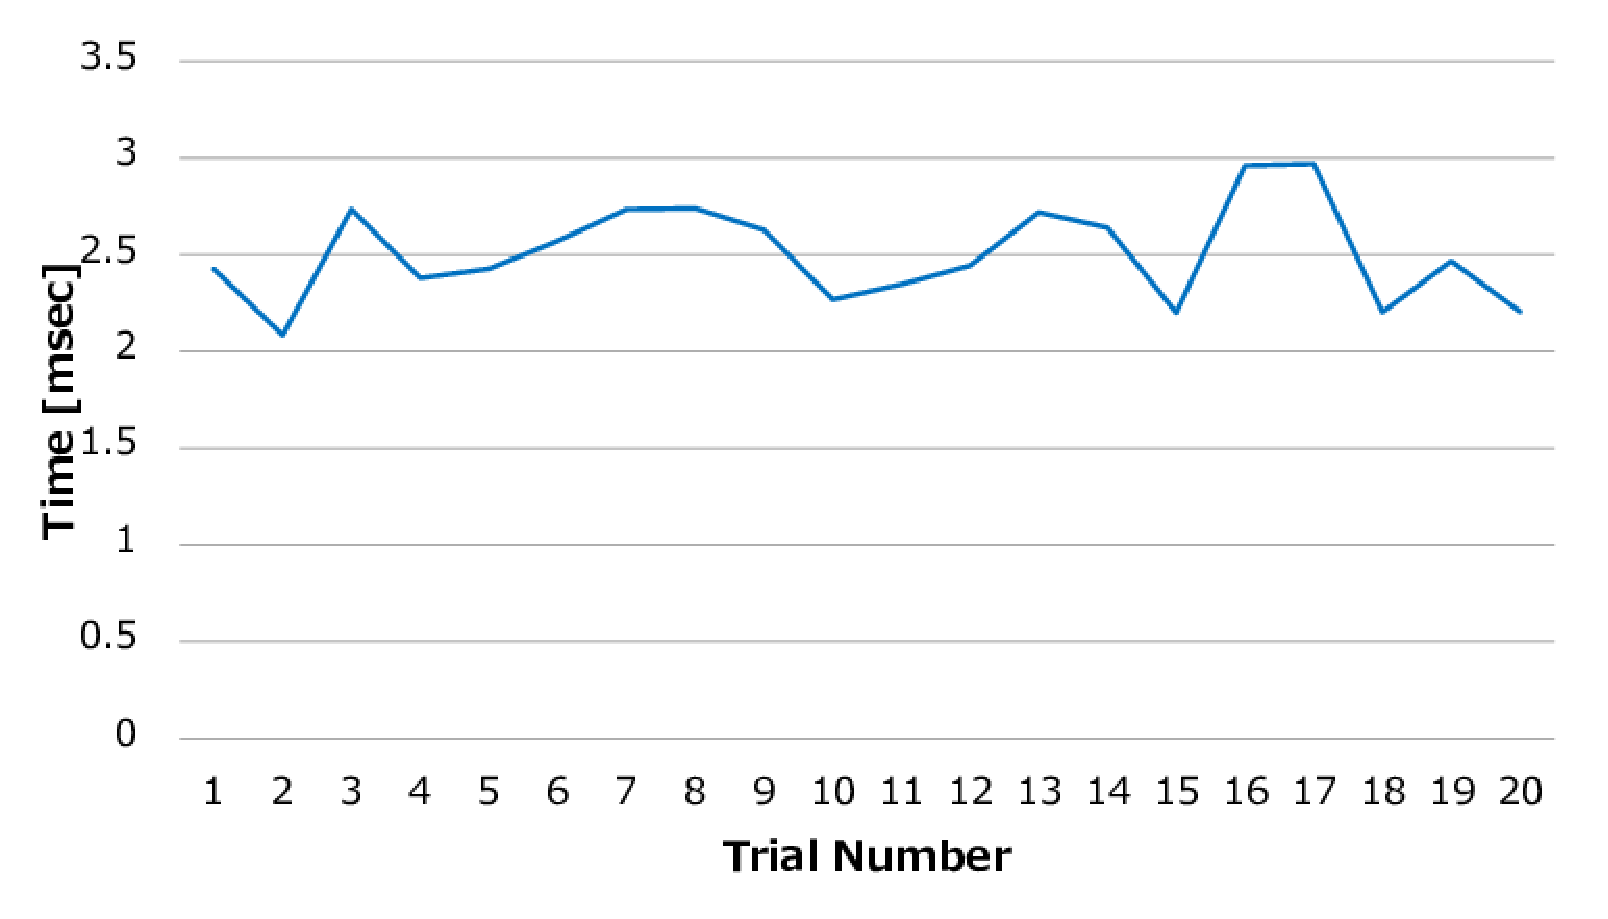
\includegraphics[width=8cm,clip]{figure/eval_synchronization.eps}
    \vspace{1mm}
\caption{Synchronization of four RiteVM tasks}
    \vspace{1mm}
\label{fig:eval_synchronization}
\end{figure}

\subsection{Benefits of component-based development}
In the proposed framework, RiteVMs, RiteVM scheduler, and Eventflags are implemented as TECS components.
Developers can easily add or remove the functionalities by modifying the CDL file.
Moreover, component-based development decreases code sizes and improve productivity and maintainability.
\DIFdelbegin \subsubsection{\DIFdel{Code size utilizing component-based development}}
%DIFAUXCMD
\addtocounter{subsubsection}{-1}%DIFAUXCMD
\DIFdelend \DIFaddbegin 

%DIF > \subsubsection{Code size utilizing component-based development}
\DIFaddend To indicate the superior of component-based development, the comparison of code lines between two C and CDL files is shown in Table \ref{tab:codesize}.
(A) and (B) mean the source files in the upper and lower of Figure \ref{fig:Eventflag}, respectively. 
In terms of C, (B)'s \DIFaddbegin \DIFadd{code }\DIFaddend lines do not increase even if the number of RiteVMs increases, while (A)'s \DIFaddbegin \DIFadd{code }\DIFaddend lines increase as the number \DIFaddbegin \DIFadd{of RiteVM }\DIFaddend increases.
(B)'s C file can be utilized without modification, regardless of the number of RiteVMs.
Moreover, \DIFaddbegin \DIFadd{code }\DIFaddend lines of two CDL files are equal.
The skillful component-based development brings this advantages such as the decrease of code lines and non-modified code, which leads high productivity and high maintainability.

\begin{table}[t]
    \centering
    \vspace{1mm}
\caption{\DIFaddbeginFL \DIFaddFL{Code }\DIFaddendFL Lines of C and CDL file for the number of RiteVM}
    \vspace{1mm}
    %\scriptsize
    {\tabcolsep=0.2cm
    \begin{tabular}{c||c|c|c}
                & (A)       & (B)     & Diff  \\ \hline
        C (Total)      & 8$\times$$\alpha$$+$134  & 130     & 8$\times$$\alpha+$4\\
        C (Modification)   & 10$\times\alpha$$-$2 & 0   &  10$\times\alpha$$-$2 \\
        CDL    & 18$\times$$\alpha$$+$25   & 18$\times$$\alpha$$+$25 & 0     \\
        \multicolumn{3}{l}{{\small $\alpha$} : {\scriptsize the number of RiteVM}}
    \end{tabular}
    }
    \label{tab:codesize}
\end{table}

\section{Related Work}
\label{sec:Related work}

\begin{table*}[t]
    \centering
    \vspace{1mm}
\caption{Comparison of the proposed and previous work}
    \DIFdelbeginFL %DIFDELCMD < \vspace{1mm}
%DIFDELCMD <     %%%
\DIFdelendFL \DIFaddbeginFL \vspace{2mm}
    \DIFaddendFL %\scriptsize
    {\tabcolsep=0.05cm
    \begin{tabular}{c||c|ccccccc}
        & Bluetooth Loader & \shortstack{Call\\C Function} & \shortstack{Legacy Code of\\Embedded System} & \shortstack{VM\\Management} & \shortstack{VM\\Scheduler} & \shortstack{Synchronization of\\Applications} & Co-routine \\ \hline
        python-on-a-chip \cite{url:python-on-a-chip} &            &            &            &            &             &            & \checkmark \\
        Owl system \cite{par:owl}                    &            & \checkmark & Partially  &            &             &            & \checkmark \\
        eLua \cite{url:eLua}                         &            & \checkmark & Partially  &            &             &            & \checkmark \\
        \DIFaddbeginFL \DIFaddFL{Squirrel \mbox{%DIFAUXCMD
\cite{url:Squirrel}                 }%DIFAUXCMD
}&            & \checkmark &            &            &             &            & \checkmark \\
        \DIFaddendFL mruby \cite{par:mruby}                       &            & \checkmark &            &            &             &            & \checkmark \\
        mruby on TECS \cite{par:mrubyonTECS}         &            & \checkmark & \checkmark & \checkmark &             &            & \checkmark \\
        Proposed framework                           & \checkmark & \checkmark & \checkmark & \checkmark & \checkmark  & \checkmark & \checkmark \\
    \end{tabular}
    }
    \label{tab:comparison}
\end{table*}
The open-source run-time systems for scripting languages have been proposed such as follow:
python-on-a-chip \cite{url:python-on-a-chip}, the Owl system \cite{par:owl}, eLua \cite{url:eLua}, \DIFaddbegin \DIFadd{Squirrel \mbox{%DIFAUXCMD
\cite{url:Squirrel}}%DIFAUXCMD
, }\DIFaddend mruby \cite{par:mruby}, \cite{url:mruby}, and mruby on TECS \cite{par:mrubyonTECS}.

\DIFaddbegin {\mybf \DIFaddend python-on-a-chip\DIFaddbegin \DIFadd{:}} \DIFadd{python-on-a-chip }\DIFaddend (p14p) is a Python run-time system that uses a reduced Python VM called PyMite.
The VM runs a significant subset of Python language with few resources on a micro-controller.
p14p can run multiple stackless green threads.

\DIFaddbegin {\mybf \DIFadd{Owl system:}} \DIFaddend The Owl system is an embedded Python run-time system.
The Owl is a complete system for ARM Cortex-M3 micro-controllers.
The Owl toolchain produces relocatable memory images, that are directly runnable on the micro-controller, from Python code objects.
The interpreter of the Owl system is the same as that of python-on-a-chip.

\DIFaddbegin {\mybf \DIFadd{eLua:}} \DIFaddend eLua offers the full implementation of Lua programming language to the embedded systems.
Lua is one of the most popular script languages for embedded systems \cite{url:Lua}, \cite{par:Lua}.
Lua supports co-routine, referred to collaborative multitasking.
A co-routine in Lua is used as an independently executed thread.
A co-routine can just suspend and resume multiple routines.
Thus, a Lua co-routine is not like multitasks in multitask systems.

\DIFaddbegin {\mybf \DIFadd{Squirrel:}} \DIFadd{Squirrel is object-oriented programming language, designed to be a lightweight scripting language that fits in real-time requirements of applications.
Squirrel is inspired by especially Lua.
The API is very similar to Lua and the table code is based on the Lua one.
Squirrel also supports co-routine as well as Lua.
}

{\mybf \DIFadd{mruby:}} \DIFaddend mruby, the lightweight implementation of the Ruby language, has been proposed for embedded systems.
mruby programs can run on a RiteVM, which is the VM for mruby and reads the mruby bytecode.
RiteVM supports only single thread.
mruby has supported co-routine, but not supported multitasking for RTOSs.

\DIFaddbegin {\mybf \DIFaddend mruby on TECS\DIFaddbegin \DIFadd{:}} \DIFadd{mruby on TECS }\DIFaddend is a component-based framework for running mruby programs.
The programs on mruby on TECS can execute about 100 times faster than the mruby programs.
Software can be also developed with component base by mruby on TECS.
Although multitasking has been supported in the current mruby on TECS, developers need to be familiar with functions of an RTOS to use multitasking.
The co-routine is supported as same as mruby.

Table \ref{tab:comparison} shows a comparison between the proposed framework and previous work.
The proposed framework supports the loader, the VM scheduler, and synchronization of application.

% In addtion, there are component systems for embedded systems.
% AUTOSAR (AUTomotive Open System ARchitecture) \cite{} is a worldwide development partnership of vehicle manufactures.
%
% SaveCCM \cite{par:SAVEapproach} is a component model for embedded control application.
% SaveCCM is a simple model which is flexible to facilitate analysis of real-time and dependability.
%
% Koala \cite{par:Koala} is a component model that helps to manage the growing complexity and diversity of software in consumer electronics products.


\section{Conclusion}
\label{sec:Conclusion}
This paper has presented an extended framework of mruby on TECS:
\DIFdelbegin \DIFdel{mruby bytecode loader using Bluetooth }\DIFdelend \DIFaddbegin \DIFadd{Bluetooth loader for mruby bytecode }\DIFaddend and RiteVM scheduler.
The loader provides developers with the software development efficiency without rewriting a storage/ROM device and restarting an \DIFdelbegin \DIFdel{OS}\DIFdelend \DIFaddbegin \DIFadd{RTOS}\DIFaddend .
The proposed framework can be applied to many kinds of embedded systems  because the loader can use not only Bluetooth also wired serial connection.
%Thus, the proposed framework can be utilized on the devices without Bluetooth.
The RiteVM scheduler makes multitasking more easily than the current mruby on TECS.
In the evaluation, experimental results of the loader and the RiteVM scheduler show their advantages.
The loader can improve the software development efficiency on mruby on TECS.
The RiteVM scheduler has the effectiveness in terms of execution time and ease of use compared with singletasking and co-routine.
%because of the low overhead.
In addition, synchronization of multiple RiteVM tasks is implemented.

The proposed framework is developed in component-base by TECS.
The facilities such as RiteVMs, the RiteVM scheduler, and Eventflag are implemented as components.
Therefore, developers can easily add or remove the functionalities as necessary, and also reuse them.
Developers can choose fair scheduling or fixed-priority scheduling since the RiteVM scheduler can be easily added and removed.
When software in priority-based scheduling is developed, developers only have to remove the RiteVM scheduler.
Component-based development can increase productivity.

Our prototype system and application programs used in the performance evaluation are all open-source, and may be downloaded from our website \cite{url:download}.

In the future, the CDL files for RiteVM and mruby-TECS bridge are generated automatically using a plugin, and developers can send a bytecode with ZMODEM protocol on the command line.
Moreover, we will support mruby libraries to mrbgems, which is a distribution packaging system for mruby.

%%%%%%%%%%%% Acknowledgement %%%%%%%%%%%%%%%%%%%%%%%%%%%%%%%%%%%%%%%%
\section{Acknowledgement}
This work was supported by JSPS KAKENHI Grant Number 15H05305.
We would like to thank Takuya Ishikawa, Hiroshi Mimaki, and Kazuaki Tanaka for supporting this research.
%%%%%%%%%%%% Reference %%%%%%%%%%%%%%%%%%%%%%%%%%%%%%%%%%%%%%%%%%%%%%
\bibliographystyle{abbrv}
\bibliography{ref}

\end{document}
